\documentclass[12pt,a4paper]{book}



		% --------------------------------- 페이지 스타일 지정
		\usepackage{geometry}
%		\geometry{landscape=true	}
		\geometry{top 		=10em}
		\geometry{bottom		=10em}
		\geometry{left		=8em}
		\geometry{right		=8em}
		\geometry{headheight	=4em} % 머리말 설치 높이
		\geometry{headsep		=2em} % 머리말의 본문과의 띠우기 크기
		\geometry{footskip		=4em} % 꼬리말의 본문과의 띠우기 크기
% 		\geometry{showframe}
	
%		paperwidth 	= left + width + right (1)
%		paperheight 	= top + height + bottom (2)
%		width 		= textwidth (+ marginparsep + marginparwidth) (3)
%		height 		= textheight (+ headheight + headsep + footskip) (4)


			\usepackage[hangul]{kotex}				% 한글 사용
			\usepackage[unicode]{hyperref}	% 한굴 하이퍼링크 사용
			\usepackage{amssymb,amsfonts,amsmath}% 수학 수식 사용
			
			\usepackage{enumerate}			%
			\usepackage{enumitem}			%
			\usepackage{pifont}				%
			\usepackage{setspace}			%
			\usepackage{booktabs}			% table
			\usepackage{color}				%
			\usepackage{multirow}			%
			\usepackage{boxedminipage}		% 미니 페이지
			\usepackage[pdftex]{graphicx}	% 그림 사용
			\usepackage[final]{pdfpages}	%pdf 사용
			\usepackage{framed}	%pdf 사용





		% ----------------------------- 장의 목차
			\usepackage{minitoc}
			\setcounter{minitocdepth}{4}    	% Show until subsubsections in minitoc
			\setlength{\mtcindent}{12pt} 	% default 24pt
	
	
		% --------------------------------- 페이지 스타일 지정
			
			\usepackage[Bjornstrup]{fncychap}
		
		
			\usepackage{fancyhdr}
			\pagestyle{fancy}
			\fancyhead{} % clear all fields
			\fancyhead[LO]{\small \leftmark}
			\fancyhead[RE]{\small \leftmark}
			\fancyfoot{} % clear all fields
			\fancyfoot[LE,RO]{\large \thepage}
			%\fancyfoot[CO,CE]{\empty}
			\renewcommand{\headrulewidth}{0.4pt}
			\renewcommand{\footrulewidth}{0.4pt}
	
		% --------------------------------- 	section 스타일 지정
	
		\usepackage{titlesec}
		
		\titleformat*{\section}			{\large\bfseries}
		\titleformat*{\subsection}			{\normalsize\bfseries}
		\titleformat*{\subsubsection}		{\normalsize\bfseries}
		\titleformat*{\paragraph}			{\normalsize\bfseries}
		\titleformat*{\subparagraph}		{\normalsize\bfseries}
	
		\renewcommand{\thesection}			{\arabic{section}.}
		\renewcommand{\thesubsection}		{\thesection\arabic{subsection}.}
		\renewcommand{\thesubsubsection}	{\thesubsection\arabic{subsubsection}}
		
		\titlespacing*{\section} 			{0pt}{1.0em}{2.0em}
		\titlespacing*{\subsection}	  		{0ex}{1.0em}{1.0em}
		\titlespacing*{\subsubsection}		{0ex}{1.0em}{1.0em}
		\titlespacing*{\paragraph}			{0ex}{1.0em}{1.0em}
		\titlespacing*{\subparagraph}		{0ex}{1.0em}{1.0em}
	
	%	\titlespacing*{\section} 			{0pt}{0.0\baselineskip}{0.0\baselineskip}
	%	\titlespacing*{\subsection}	  		{0ex}{0.0\baselineskip}{0.0\baselineskip}
	%	\titlespacing*{\subsubsection}		{6ex}{0.0\baselineskip}{0.0\baselineskip}
	%	\titlespacing*{\paragraph}			{6pt}{0.0\baselineskip}{0.0\baselineskip}
	

		% --------------------------------- recommend		섹션별 페이지 상단 여백
		\newcommand{\SectionMargin}			{\newpage  \null \vskip 0cm}
		\newcommand{\SubSectionMargin}		{\newpage  \null \vskip 0cm}
		\newcommand{\SubSubSectionMargin}	{\newpage  \null \vskip 0cm}


	
		% --------------------------------- 장의 목차
		\usepackage{minitoc}
		\setcounter{minitocdepth}{1}    	% Show until subsubsections in minitoc
		\setlength{\mtcindent}{12pt} 		% default 24pt
	
	
		% --------------------------------- 	문서 기본 사항 설정
		\setcounter{secnumdepth}{3} 		% 문단 번호 깊이
		\setcounter{tocdepth}{2} 			% 문단 번호 깊이
		\setlength{\parindent}{0cm} 		% 문서 들여 쓰기를 하지 않는다.
		
		
		% --------------------------------- 	줄간격 설정
		\doublespace
%		\onehalfspace
%		\singlespace






		% --------------------------------- recommend  글자 색깔지정 명령
		\newcommand{\red}		{\color{red}}			% 글자 색깔 지정
		\newcommand{\blue}		{\color{blue}}		% 글자 색깔 지정
		\newcommand{\black}	{\color{black}}		% 글자 색깔 지정
		\newcommand{\superscript}[1]{${}^{#1}$}







% 	============================================================================== List global setting
%		\setlist{itemsep=1.0em}
	
% 	============================================================================== enumi setting

	%	-------------------------------------------------------------------------------
	%		Vertical and Horizontal spacing
	%	-------------------------------------------------------------------------------
		\setlist[enumerate]	{ 	itemsep=0.0em, 
								leftmargin=6.0ex, 
								rightmargin=0.0em, 
								labelwidth=0.0em, 
								labelsep=4.0ex 
							}

	%	-------------------------------------------------------------------------------
	%		Label
	%	-------------------------------------------------------------------------------
		\setlist[enumerate,1]{ label=\textbf{(\arabic*)}, ref=\textbf{(\arabic*)} }	% (1)
		\setlist[enumerate,2]{ label=\textbf{\arabic*)}, ref=\textbf{\arabic*)} }		% 1)
		\setlist[enumerate,3]{ label=\textbf{\arabic*.}, ref=\textbf{\arabic*.} }		% 1.

% 	============================================================================== itemi setting

	%	-------------------------------------------------------------------------------
	%		Vertical and Horizontal spacing
	%	-------------------------------------------------------------------------------
		\setlist[itemize]{itemsep=0.0em}



% --------------------------------- 환경 정의 : 박스 치고 안의 글자 빨간색

			\newenvironment{BoxRedText}
			{ 	\setlength{\fboxsep}{12pt}
				\begin{boxedminipage}[c]{1.0\linewidth}
				\color{red}
			}
			{ 	\end{boxedminipage} 
				\color{black}
			}


\begin{document}

% ------------------------------------------------------------------------------
% Maketitle
% ------------------------------------------------------------------------------
			\begin{titlepage}
			\thispagestyle{empty}				% Remove page numbering on this page
			\definecolor{grey}{rgb}{0.9,0.9,0.9} 
			\colorbox	{grey}
						{ \parbox[t]{1.0\linewidth}
						{
						\vspace*{1.2cm} 
						\fontsize{20}{20} \rmfamily \hfill \today 		\\ [0.4cm] \null
						\fontsize{40}{20} \rmfamily \hfill 한국의 지질\\ [0.4cm] \null
						\fontsize{20}{50} \rmfamily \hfill ver101
						\vspace*{0.8cm} 
						} }
			\vfill
			% Print the author data as defined above
			\hfill Kim Dae Hee\\ \null
			\hfill (주)서영엔지니어링\\ \null
			\hfill 건설관리팀\\ \null
			\hfill \url{h01038395609@gmail.com} \\ \null
			\hfill \rule{0.4\linewidth}{1pt}
			\end{titlepage}																														\clearpage
% ------------------------------------------------------------------------------
% 
% ------------------------------------------------------------------------------


			% ----------------------- 장 목차 생성 Initialization
			\dominitoc		
			
			% ----------------------- 장 목차 생성 Initialization
			\tableofcontents
			\listoffigures
			\listoftables
	
	

% ===========================================================	part		=============
		\addtocontents{toc}{\protect\newpage}
		\part{한반도의 지질 개관}

% ========================================== chapter ============ 트리즈
\newpage
\chapter{한반도의 지질 개관}



	\SectionMargin
	\section{	한반도의 지질 개관}


			한반도는 국토의 반 이상이 【 화강암 】과 【 화강편마암 】으로 되어 있다. 
			\\[-1.0em]

			전자는 대체로 트라이아스기쥬라기백악기에 관입한 것이고, 후자는 그 대부분이 선캠브리아누대의 퇴적암이 화강암화작용으로 변성된 것이다.

			이들은 여러 시기의 지각변동과 제3기 초부터 일어난 한반도의 융기작용과 삭박작용으로 지표에 노출하게 되었다.  
			그러므로 퇴적암류는 편마암위에 분포한다.


	\SectionMargin
	\section{	시대별 지역별 분포}


			이들 암석의 시대별 및 지역별 분포의 모양을 요약하면 다음과 같다, 

			여기서 남한 및 북한의 구별은 지질학적인 것으로서 서울-원산선을 그 경계로 하며, 정치적인 의미를 가진 용어는 아니다.

			\begin{enumerate}
			\item[1)] 	선캠브리아누대의 것으로 생각되는 변성퇴적암의 주요 분포지는 한반도 중부에 있다.
			\item[2)] 	두 개의 큰 고생대층 분포지는 평안남도와 강원도 북부에 있다.
			\item[3)] 	비교적 큰 중생대층의 분포지는 경상남북도에 있고 작은 노출지들은 충청남도 중서부와 평양 부근에 있다.
			\item[4)] 	제3계의 작은 분포지는 동해안에 따라 몇 곳에서, 서해안에서는 두 곳에서 발견된다.
			\item[5)] 	북한에는 화강암의 저반이 거의 무질서하게 곳곳에 분산되어 있으나 
						남한에서는 북북동-남남서의 지나방향에 관계있는 분포 상태를 보여 주며, 분포 면적과 저반의 규모가 크다.
			\item[6)] 	제4기의 화산암은 백두산 부근반도 중앙부동남 해안제주도울릉도에서 발견된다.
			\item[7)] 	지층의 특징으로서는 해성층이 적고 육성층이 많은 사실을 들 수 있다. 
						즉 고생대 전반까지의 지층은 대체로 해성층이나 고생대 말엽의 지층의 대부분중생층의 전부신생층의 약 절반은 육성층에 속한다.
			\end{enumerate}




% ========================================== chapter ============ 트리즈
\newpage
\chapter{한국 지질 계통명}








% ========================================== chapter ============ 트리즈
\newpage
\chapter{한반도의 지각변동}

	% -------------------------------------- page -------------------
		%			\nomtcrule         		% removes rules = horizontal lines
		%			\nomtcpagenumbers  % remove page numbers from minitocs
					\minitoc				% Creating an actual minitoc
		


	% ------------------------------------------ section ------------ 
	\SectionMargin
	\section{한반도의 지각변동}

		【 고생대 】이후 오랜 기간 침식을 받아 저평화된 한반도는 
		【 중생대 】로 접어들면서 지각이 크기 요동치며 휘어지거나 단절되고, 
		또 지각의 일부가 내려앉거나 솟아오르는 등 전국적으로 거대한 규모의 지각 변동을 겪었다. \\

		그 결과 지각 깊은 곳에 있던 마그마가 화산폭발로 지표에 분출되기도 하고, 
		또 일부는 지각의 약한 틈을 뚫고 솟아오르다가 지하 깊은 곳에서 냉각, 고화되기도 했다. \\

		지표로 분출된 마그마인 용암이 굳으면 현무암이 되고, 
		지하 깊은 곳에 관입하여 굳으면 심성암이 된다. 
		금강산을 이루는 암석은 바로 중생대에 여러 차례 관입한 심성암 가운데 하나인 화강암이다. 
		화강암은 우리나라 산지의 30\%를 차지하는 암석으로 
		오랜 기간 침식과 풍화를 받아 지금의 수석 전시장 같은 풍경을 만들어냈다.
	
	



% ===========================================================	part		=============
		\addtocontents{toc}{\protect\newpage}
		\part{한반도의 형성}


% ========================================== chapter ============ 트리즈
\newpage
\chapter{한반도의 형성}

	% -------------------------------------- page -------------------
		%			\nomtcrule         		% removes rules = horizontal lines
		%			\nomtcpagenumbers  % remove page numbers from minitocs
					\minitoc				% Creating an actual minitoc
		
	
	
	

	% ------------------------------------------ section ------------ 
	\SectionMargin
	\section{한반도의 형성}
	\null



			\Large 
			오스트레일리아 서쪽에 붙어 있다가 중생대 【 쥐라기 】에 현재 위치에 도달
			\normalsize \\
			
			\red
			【 고생대 초 】에 한반도는 지금의 위치가 아니라 적도 이남 10 부근에 있다가 
			점차 북상하여 【 중생대 트라이아스기 】에 북위 25에 도달했으며, 
			약 2억 년 전 【 쥐라기 】에 이르러 지금의 38 부근에 도달했다.
			\black \\
			


약 5억 년( 5.7억 년 ) 전 고생대에는 한반도는 남위 35 부근의 오스트레일리아 서쪽에 붙어 있었다. 
오늘날 강원도 영월, 태백 지역에 많이 분포하는 석회암은 한반도가 열대의 얕은 바다 속에 있었을 때 형성된 암석이다. 
이후 한반도는 대륙에서 분리되어 점차 북쪽으로 이동하기 시작했으며, 약 3억 년 전에는 적도 부근까지 올라왔다. 
그리고 약 2억 년 전 중생대 쥐라기에 지금의 위치인 북반구 중위도에 이르게 되었다.
\\[-1.0em]

놀랍게도 약 2억년 전 한반도는 원래 2개의 땅덩어리였던 것이 결합하여 하나가 되었다. 
오스트레일리아에서 올라온 남부 땅덩어리와 중국에 붙어 있던 북부 땅덩어리가 쥐라기때 충돌하면서 하나가 되었는데, 
이때의 충격으로 한반도 전역에 대규모 지각 변동이 일어났다. 
우리나라의 지형과 지질이 가장 큰 격변을 겪은 것은 바로 이때였다. 
지질학자들은 그 충돌대가 임진강 일대라고 추측한다, 
왜냐하면 임진강 일대는 북중국과 남중국의 친링~다비~산둥선과 연결되었을 가능성이 높기 때문이다.
\\[-1.0em]

한편 10여년 전 ``한반도가 매년 $2 \sim 3 cm$씩 동쪽으로 이동하고 있다''는 가설이 제기된 적이 있다. 
일본 국립천문대와 국토지리정보원이 인공위성으로 측정한 결과, 
유라시아 대륙판에 속해 있는 한반도와 만주지방, 그리고 일본 열도 서남부가 아무르판이라는 새로운 판 위에 놓여 있을 가능성이 컸다. 
아므르판은 아직 정식으로 확인되지 않았으나 일본 서남부 지역에 있으리라 추정되는 지각판이다. 
여기서 한반도가 속해 있는 아무르판이 동해가 속해있는 오호츠크 판 밑으로 미끄러져 들어가고 있기 때문에 
한반도가 매년 동쪽으로 수cm씩 이동하고 있다는 주장이 나왔다.
만약 이 가설이 사실이라면 3억년 넘게 지질 여행을 해온 한반도가 영원히 사라질지도 모를 일이다.
\\[-1.0em]




% ========================================== chapter ============ 트리즈
\newpage
\chapter{동해의 형성}


	% ------------------------------------------ section ------------ 
	\SectionMargin
	\section{동해의 형성}
	\null
	
			동해가 과연 어떻게 형성됐는지는 이직도 논쟁이 계속되고 있는 주제이다.
			\\[-1.0em]

			동해는 서남해와 출생부터 다르다. 
			서남해가 간빙기 해수면이 높이지면서 물에 잠긴 육지라면, 동해는 지각이 깊게 갈라지고 그 틈새에 해양 지각이 형성돼 만들어진 바다다.
			\\[-1.0em]

			\paragraph{한국대지}
			일본이 한반도에서 분리되면서 떨어져 나간 육지 조각은 지각변동의 흔적으로 동해에 널려 있다. 
			울릉도 북쪽에 위치한 한국대지가 그 하나이다. 
			폭 250km, 길이 200km의 넓은 해저 대지인 이곳의 수심은 주변이 2,000m가 넘는데 견줘 800m도 안 되는 곳이 있울 정도로 상대적을 얕다. 
			한국대지에서 굴착한 암석은 북한산이나 설악산을 이루는 암석과 비슷한 중생대 쥐라기의 대보화강암인 것으로 나타났다.
			\\[-1.0em]



3. 		동해의 형성

지각은 북극 바다에 떠 있는 거대한 얼음평상(빙상)과 비슷하다. 
얼음이 떨어져나가 무게가 가벼워지면, 얼음장은 새로운 무게 중심을 잡기 위해 상승한다. 북유럽의 영국이나 스칸디나비아 반도는 그런 예이다. 지난 빙하기 때 두꺼운 얼음에 덮여 눌러있던 스칸디나비아 반도는 얼음이 녹아 무게가 가벼워지면서 그 반작용으로 현재 한반도의 100배인 100년에 1m꼴로 땅이 솟아오르고 있다. 

영국은 빙하에 덮였던 북부 지방의 얼음이 녹으면서 북구가 상승하자 그 반작용으로 런던 등 남부 지방은 가라앉는 현상이 벌어지고 있다. 

일본이 떨어져 나간 한반도 땅 덩어리가 새롭게 무게 중심을 잡느라 기우뚱하면서 솟아오른 곳이 바로 태백산맥이다. 태백산맥은 현재도 융기운동을 계속하고 있다. \\

폭포는 한반도 융기의 증거이다. 땅이 솟아오르면 물살이 빨라져 침식을 가속한다. 이런 침식의 선단이 바로 폭포이다, 이 때문에 폭포는 쉬지 않고 뒤로 물러선다. 폭포 끄트머리 암반이 침식해 사라지기 때문이다. 강원도 삼척시 통리 협곡에 있는 미인폭포는 대표적인 예이다. 중생대 백악기의 퇴적층이 고생대 석탄지대로 둘러싸여 있는 통리협곡은 상대적으로 무른 퇴적층이 300m 가까이 패여 붉은 퇴적 암반이 드러난 깊은 계곡이 됐다. 협곡을 흐르는 오십천은 동해가 열리고 태백산맥이 솟으면서 물살리 빠라져 침식을 가속했다. 상류로 향하는 이 침식의 끝자락이 바로 미인폭포이다.




		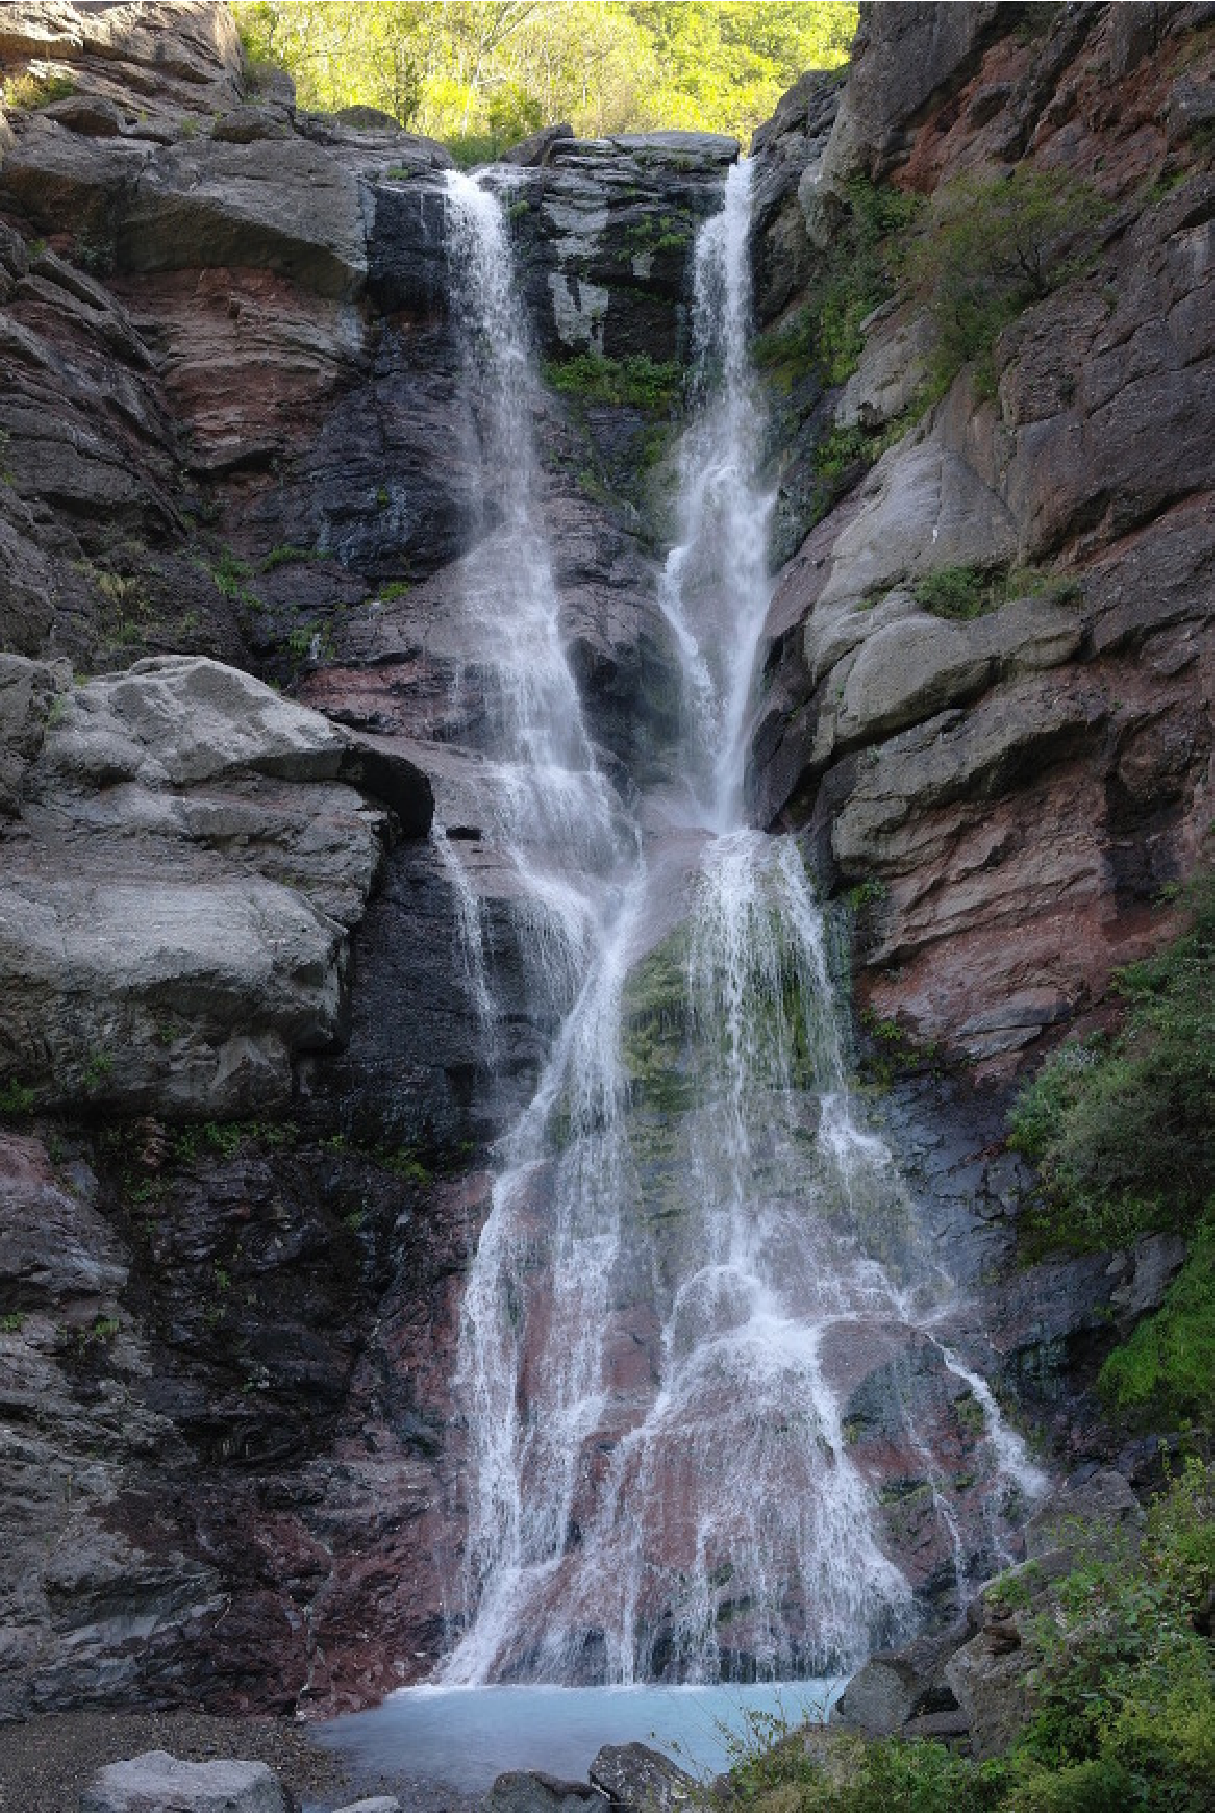
\includepdf[pages=-, fitpaper=true ]{./fig/SAM_9717.pdf}



	% ------------------------------------------ section ------------ 
	\SectionMargin
	\section{부채꼴 확장설}
	\null




		\subsection{한반도, 10만년에 10m꼴 융기}

		강원도 강릉의 정동진 해안은 해돋이 관광객뿐 아니라 지형학자에게도 명소이다. 
		한반도의 땅덩어리가 솟아오른 가장 도드라진 증거가 여기 펼쳐져 있기 때문이다.
 
		모래시계공원이 있는 해변에서 조각공원 쪽을 바라보면, 언덕 위에 올라앉은 배 모양의 리조트 건물이 이채롭다. 
		그러나 60만$\sim$70만년 전 이 `배'가 있는 평평한 언덕은 실제로 파도가 치는 해수면이었다. 
		\\[-1.0em]
 




 
		장호 전북대 지리교육과 교수는 “썬크루즈 리조트가 있는 해발 60$\sim$70m의 해안단구는 정동진에서 가장 넓은 단구”라며 
		``정동진에는 해발 160m까지 약 10m 높이마다 단구 면이 나타난다''고 말했다.
 
		그는 ``한반도의 땅덩어리는 1000년에 0.1m, 곧 10만 년에 10m꼴로 융기하고 있다''며 
		``정동진은 그런 융기를 보여주는 교과서 같은 증거''라고 설명했다.
 
		해안단구는 파도에 깎여 평평해진 해안이 지반융기와 함께 솟아올라 형성된다. 
		정동진에서는 심곡리 곰두리 단구에서 바위에 구멍을 파는 조개화석이 발견됐는가 하면 
		해발 160m 단구에서 암반이 파도에 깎여 만들어진 자갈층이 확인되기도 했다.
 


		한반도 융기의 또 다른 주요 증거는 산꼭대기의 평평한 땅을 가리키는 고위평탄면이다. 
		해발 1300m인 대관령 삼양목장과 800m인 횡성휴게소, 500m인 남한산성을 이으면 한 직선상에 놓인다.
 
		최성길 공주대 사범대학장(지형학)은 “이들 세 지점은 과거에 하나의 평탄면, 
		곧 해수면을 이뤘다”며 “신생대 말 지반운동을 받아 동해안 쪽이 서해안 쪽보다 더 많이 솟아올라 현재의 ‘동고 서저’ 지형을 이뤘다”고 설명했다.
		\\[-1.0em]

 
		\subsection{박수진 서울대 지리학과 교수는 }
		한반도가 지역별로 다양한 융기를 보인다는 주장도 있다. 
		박수진 서울대 지리학과 교수는 수치고도모델(DEM)로 한반도의 지형을 분석해 북부·중부·남부·동해안 등 4개 지반운동구로 나눴다. 
		융기의 중심은 개마고원과  태백산맥, 덕유산·지리산 축이었다.
 
		박 교수는 “신생대 제3기 단층운동으로 태백산맥과 개마고원을 중심으로 북서쪽으로 기운 한반도 지형의 원형이 형성됐고, 
		이후엔 산지가 침식되면서 줄어든 무게를 보상하기 위한 지각균형적인 점진적 융기가 일어나고 있다”고 밝혔다.
 
		최 교수도 “한때 서·남해안의 복잡한 해안선을 침강으로 설명한 적이 있었지만 
		이곳에서도 해안단구가 잇따라 발견되면서 융기가 분명해졌다”며 “약 200만 년 전 이후에는 동·서해안의 융기속도가 같아졌다”고 말했다.
 


		동해 바닥에서 발견된 ‘육지 조각’
 
		그렇다면, 한반도에 산맥이 솟고 지형이 동쪽으로 기울게 한 원동력은 무엇일까. 
		지질학자들은 그 힘이 신생대 제3기 동안 동해를 열고 일본이 한반도에서 떨어져 나가도록 했다고 믿는다.
 
		먼저, 동해와 태백산맥의 형성이 비슷한 시기에 일어났음을 보여준 주목할 연구결과가 나왔다. 
		민경원 플로리다대 교수와 조문섭 서울대 교수 등은 지난해 미국지구물리학연맹(AGU)에 낸 논문에서 
		대관령 화강암 내 인회석의 형성시기를, 동해 형성 시점과 같은 약 2300만 년 전으로 계산했다. 
		조 교수는 “(이로써) 동해가 처음 열리면서 경동 요곡작용에 의해 태백산맥이 만들어졌다는 기존의 가설이 지질학적으로 뒷받침된다”고 밝혔다.
 
		동해는 서·남해와 출생부터 다르다. 
		서·남해가 간빙기 해수면이 높아지면서 물에 잠긴 육지라면, 동해는 지각이 깊게 갈라지고 그 틈에 해양지각이 형성돼 만들어진 바다이다.
 
		일본이 한반도에서 분리되면서 떨어져 나간 육지 조각은 지각변동의 흔적으로 동해에 널려있다. 
		울릉도 북쪽에 위치한 한국대지는 그런 예이다. 
		폭 250㎞, 길이 200㎞의 넓은 해저 대지인 이곳의 수심은 800~2800m로 주변보다 훨씬 얕다.
 
		한국해양연구원이 한국대지에서 굴착한 암석은 북한산이나 설악산을 이루는 암석과 비슷한 중생대 쥐라기의 대보화강암인 것으로 나타났다.
 
		\SubSectionMargin
		\subsection{부채꼴 확장설 대 이단계 확장설 논란}
 
		동해의 형성은 논쟁을 부르는 주제다. 
		대륙충돌과 해양판 확장이 얽힌 복잡한 지구조 사건이 동해를 둘러싸고 벌어졌기 때문에 명쾌한 해명이 쉽지 않다.
		\\[-1.0em]
 
		\subsubsection{부채꼴 확장설}

		1980년대 중반 일본 연구자들은 ‘부채꼴 확장설’을 발표했다. 
		\\[-1.0em]

		약 1500만 년 전 일본 서남부가 대한해협을 축으로 시계방향으로 54도 회전하고, 
		동북부는 1100만$\sim$2100만 년 사이 반시계방향으로 50도 회전해 오늘날의 휘어진 일본열도와 동해를 형성했다는 이론이다.
		\\[-1.0em]
 
		김인수 부산대 지질환경과학과 교수는 “이 이론은 선풍을 일으켰지만 
		일본열도를 회전 이전으로 복원했을 때 동해에 가라앉은 대륙지각이 들어설 공간이 없고, 
		1500만 년 이전의 화산암이 동해 주변에서 발견되는 것을 설명하지 못하는 등의 한계를 지닌다”고 말했다.
 
		\subsubsection{2단계 확장설}

		‘2단계 확장설’은 부채꼴 확장 이전에 일본 섬들이 남동쪽으로 평행이동했다고 본다. <그림 참조>
		
		\begin{figure}[h!] 
		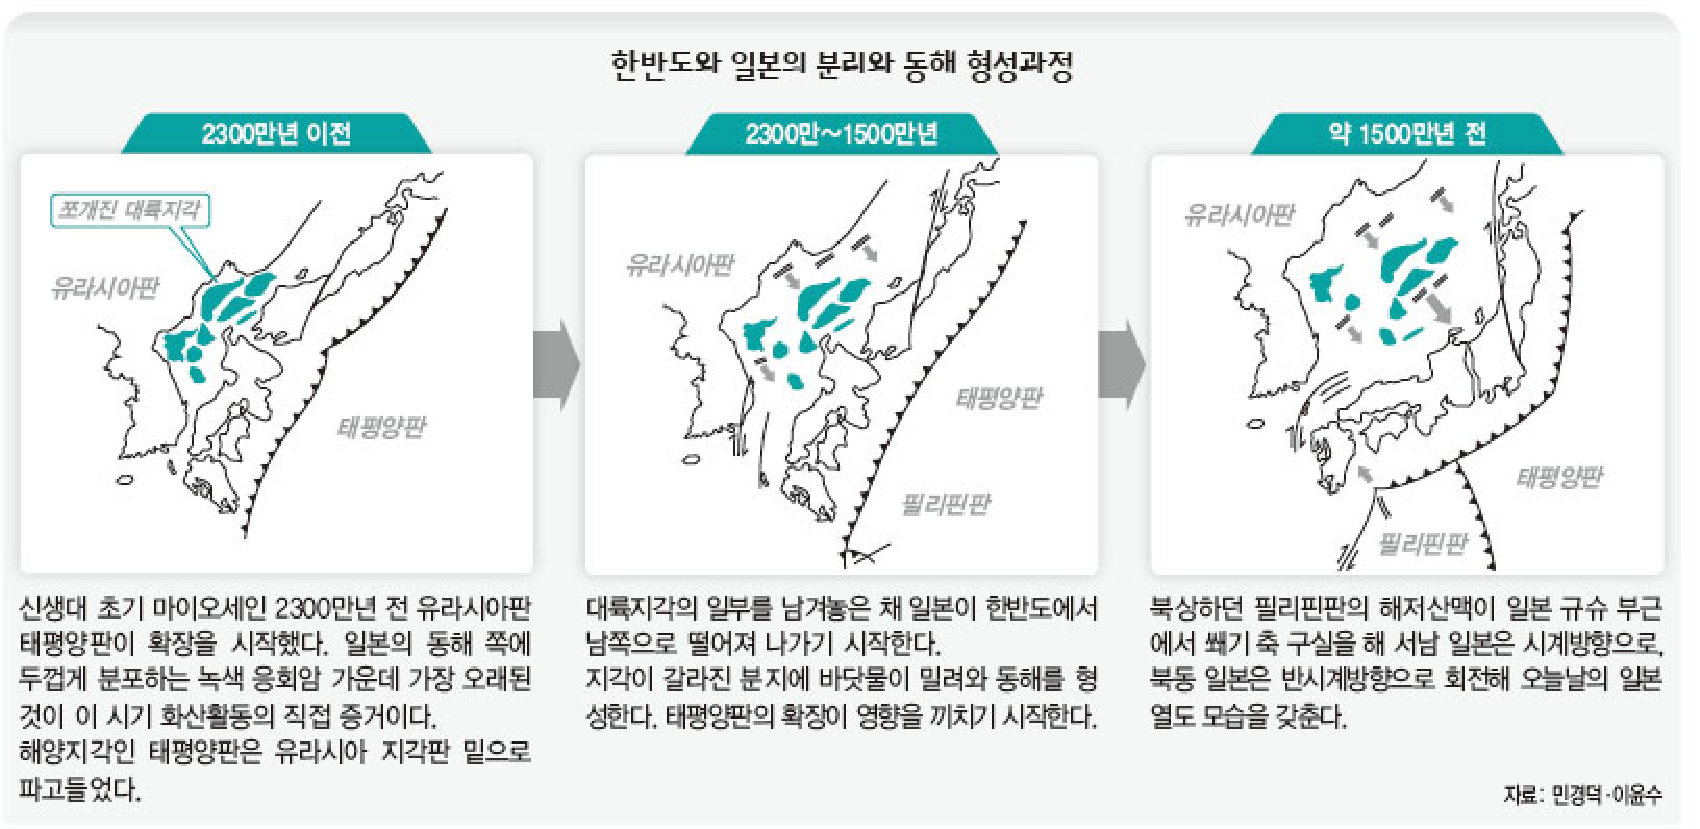
\includegraphics[width=1.0\textwidth]{./fig/rain_26690.pdf}
		\end{figure}

		\subsubsection{당겨 열림설}

		동해가 열린 원동력이 무언지도 논란거리다. 
		‘당겨열림설’은 5천만 년 전 인도대륙과 유라시아대륙의 충돌 여파로 동해가 열렸다고 본다. 
		김인수 교수는 “고무지우개를 세로로 세워 위에서 누르면 마치 양쪽에서 잡아당기듯 좌우로 벌어지는 힘이 작용한다”며 
		“그 힘 때문에 바이칼호, 남중국해와 함께 동해도 열린 것”이라고 주장했다.
 

		그러나 동해안에 탄생의 엔진이 들어있었다는 이론도 만만치 않다. 
		이윤수 한국지질자원연구원 박사는 “해양판인 태평양판이 맨틀로 파고들어 마그마를 형성하는 곳에 위치한 동해 지하는 현재도 열류량이 높다”며 
		태평양판과 필리핀판의 확장을 동해 생성의 원동력으로 꼽았다.  
 


		글·사진/조홍섭 환경전문기자 ecothink@hani.co.kr



 
		\SubSectionMargin

		◎ 뒤로 물러나는 폭포
		한반도 융기가 후퇴 가속시켜
		 
		‘한국의 그랜드캐니언’이라 불리는 강원도 삼척시 통리 협곡에 있는 미인 폭포는 대표적인 예이다.
		 
		중생대 백악기의 퇴적층이 고생대 석탄지대로 둘러싸여 있는 통리 협곡은, 
		상대적으로 무른 퇴적층이 300m 가까이 패여 붉은 퇴적암반이 드러난 깊은 계곡이 됐다.
		 
		협곡을 흐르는 오십천은 동해가 열리고 태백산맥이 솟으면서 물살이 빨라져 침식을 가속했다. 
		상류로 향하는 이 침식의 선단이 바로 미인 폭포이다.
		 
		경기도 연천군 전곡읍에 있는 재인 폭포도 물러나는 폭포의 모습을 잘 보여준다. 
		지장봉에서 흘러내린 계곡물이 한탄강의 현무암 대지를 깎아내, 현재는 강변에서 북쪽으로 350m가량 물러나 있다.
		 
		미국과 캐나다 국경의 나이아가라 폭포는 빠른 침식속도로도 유명하다. 
		이 폭포는 지난 1만 2000년 동안 11.4㎞를 후퇴해, 직선이던 폭포 선단이 말발굽 모양으로 바뀌었다. 
		연간 1m의 후퇴속도이다. 
		물흐름을 바꾸고 침식억제 공사를 통해 현재 침식속도는 연간 1㎝ 수준으로 줄었다. 
		 
		조홍섭 환경전문기자 ecothink@hani.co.kr









	% ------------------------------------------ section ------------ 
	\SectionMargin
	\section{당겨 열림설 (2단계 확장설)}
	\null
 		














	% ------------------------------------------ section ------------ 
	\SectionMargin
	\section{동해가 열린 사건}

	이윤수/한국자원연구소/이학박사
	\\[-1.0em]




"동해물과 백두산이 마르고 닳도록…" 애국가 1절에 가장 먼저 등장하는 한반도의 영역은 동해다. 바로 이 동해가 미래 한반도의 모습을 알 수 있는 열쇠다. 
\\[-1.0em]

1천만년이 지나면 동해는 현재보다 크기가 줄어들 것이고, 한반도의 동쪽 해안은 격심한 지진과 화산활동의 무대가 될 가능성이 크다. 동해는 평균 깊이가 수천m에 달하지만, 그저 밑밑하게 꺼져있는 바다가 아니다. 2천m 미만의 상대적으로 얕은 수심을 갖는 지형들이 분포하고 있다. 이 해저지형들과 함께 일본의 꺾여진 부분을 모아서 한반도의 동쪽 해안선에 끼워 맞추는 퍼즐놀이를 해보자. 그러면 놀라운 사실을 발견하게 될 것이다.
앗! 동해가 없어졌다!
그렇다. \textbf{동해는 원래 존재하지 않았으며, 약 2천3백만년 전에 새로이 탄생한 바다였던 것이다}. 즉 한반도와 일본은 하나의 육지로 연결돼 있었다는 말이다. 
독자 여러분은 2천3백만년 전이라 하면 무작정 아득히 먼 옛날로만 느껴질 것이다. 하지만 생각해보자. 어린 시절 라디오방송에 '장수만세'라는 프로그램이 있었다. 거기서 4세대가 동시에 사는 장수 집안이 소개된 기억이 있다. 조선시대의 건국시기는 불과 6백년 전으로 대개 20세대 내외에 해당하는 기간이라고 한다면, 4세대가 다섯번만 거치면 도달할 수 있는 너무 가까운 과거다. 이 6백년이 불과 17번만 거듭하면 도달하는 1만년 전의 석기시대 역시 그리 멀지 않은 옛날이며, 이 1만년을 2천3백회만 되풀이하면 동해가 막 벌어지는 시기에 도달하게 된다.
\\[-1.0em]

그렇다면 한반도에서 일본을 수제비 떼어내듯 쉽게 분리시킨 힘은 어떻게 생기는 걸까? 그 해답을 알기 위해 먼저 지표의 판구조를 살펴보자. 
지구 표면은 서로 다른 방향으로 움직이는 10여개의 주요 판들로 구성되어있다. 
현재의 한반도는 \textbf{유라시아판}에 속해 있으며, 북동쪽으로는 북아메리카판, 동쪽에는 태평양판, 남쪽에는 필리핀해판, 
그리고 서남쪽으로 인도-호주판에 둘러싸여져 있다.
\\[-1.0em]

태평양의 바닥 깊숙한 맨틀에서 솟구쳐 오르는 용암은 거대한 바다산맥(해령)을 만들고, 
그 용암이 바닷물에 식으면서 굳어져 해양지각을 만든다. 
뒤이어 생기는 새 해양지각은 바로 전에 만들어진 해양지각을 해령의 양 바깥쪽으로 밀어낸다. 
해양지각이 머나먼 지구 여행을 시작하는 것이다. 
\\[-1.0em]

멀리 밀려난 해양지각은 점점 냉각되어 비중이 커지고, 가벼운 유라시아 대륙지각을 만나면서, 유라시아판 밑으로 파고 들어가 지하 약 670 km 깊이(상부 및 하부 맨틀의 전이대)에 일시 집결된다. 이 집결체의 무게에 의하여, 뒤따라 오는 해양 지각은 마치 식탁보처럼 끌려 당기어져 들어가고, 그 결과 유라시아판과 태평양판이 만나는 경계 부위에서는 깊은 골짜기(해구)가 형성된다. 
\\[-1.0em]

해양판이 맨틀로 들어가면 어떤 일이 벌어질까? 뜨거운 맨틀층이 차가운 해양판을 달가워할 리가 없다. 마치 달구어진 기름에 감자를 넣었을 때처럼, 일대 요동이 발생하는 것이다. 더욱이 해양판 위에는 다량의 물을 포함한 퇴적물의 일부가 같이 묻어 끌려들어 가는 데, 이 수분이 맨틀의 녹는 점을 낮추어 대륙 주변에 마그마를 만든다. 이 마그마의 세력이 충분히 커지면, 더욱 강렬한 대류를 일으킨다. 이 힘에 밀려 대륙 연변부의 약한 부분이 떨어져 나갈수 있으며, 이를 후배호 확장이라 한다.
\\[-1.0em]

지도에서 보면 일본 열도는 가운데가 움푹 꺾여있는 모습을 띠고 있다. 유라시아판에서 떨어져 나갈 때 어떤 일이 벌어졌길래 이런 모습을 가지게 된 것일까. 이에 관한 3가지설이 제안되고 있다.
1980년대 일본 고베대학의 오토후지 교수는 서남일본과 동북일본에 대해 1천5백만년보다 오래된 암석들의 고지자기 방향이 같은 시대의 유라시아의 방향보다 각각 시계방향과 반시계방향으로 약 50도씩이나 차이가 난다는 중요한 연구 결과를 제시했다. 이것은 약 1천5백만년 이전에는 일본열도가 일직선상으로 놓여 있었다가 무언가의 지각 변동에 의해 서남일본과 동북일본 지괴가 각각 시계방향과 반시계방향으로 약 50도 정도 회전되었기 때문이며, 일본 열도가 굴절되었음을 의미하는 것이었다. 오토후지교수는 이 사건이 동해가 확장에서 비롯된 것으로 해석하고, 열도의 북쪽(대륙쪽)에서 후배호 확장이 동해 한가운데를 중심으로 진행되어 태평양을 향해 일본의 중앙부가 양단부에 비하여 많이 밀려났기 때문에, 오늘날과 같은 모양으로 되었다는 설명하였다. 이 모습은 마치 부채가 펼쳐진 형상과 비슷하다고 해서 '부채꼴 확장설'이란 이름이 붙여졌다. 오토후지 교수가 즐겨 찾던 술집의 문이 양쪽으로 밀고 들어가는 형태였는데, 어느 날 이 문을 열다가 힌트를 얻었다고 해서 'bar-door' 모델이라고도 불린다.
\\[-1.0em]

최근 필자는 한반도의 고지자기 연구 결과를 실시하고, 일본 열도가 꺾여지기 전에도 이미 동해가 확장되고 있었다고 제안하고, 부채꼴 확장설을 수정한 모델을 제시했다. \textbf{일본 열도가 일단 일직선으로 평행하게 밀려내려오다 어느 순간 가운데가 굽기 시작했다는 '2단계 확장설'이다}. 이 설은 필리핀해판이 시계방향으로 90 가까이 회전하면서 북상했다는 미국 남가주대학의 풀러 교수의 연구 결과 (1995년과 1996년, 영국 런던대학의 홀 교수에 의해 더욱 정밀하게 검토되었으며, 자전 방향만 반대일 뿐 동으로 휘어지는 이동 경로가 태풍과 유사)가 단서를 마련해 주었다. 
\\[-1.0em]

\clearpage

2단계 확장설을 좀더 들여다 보자. 2천3백만년 전 한반도의 동측에 위치하고 있던 일본 열도의 북측에서 후배호 확장이 일어났다. 열도는 일직선 형태로 남남동 방향으로 태평양을 향해 진행하다, 1천5백만년 전 필리핀해판이 일본 서남쪽 일대(큐우슈우)와 충돌을 일으키게 된다. 이 충돌부를 시이소오축으로 하여 일본 열도의 회전이 일어나, 지금처럼 일본이 꺾이게 되었던 것이다. 그 결과 일본 열도의 서쪽은 북상하고 동쪽은 남하하게 되었으며, 석유가스가 매장된 울산 앞바다의 주름진 지층과 단층 구조는 이때 큐우슈우가 북상하면서 만들어낸 작품이다. 
동아시아는 본디 많은 지각 조각들이 모여 모자이크처럼 복잡하게 구성된 대륙이며, 이들 경계의 이음새는 흔히 화성암이나 변성암으로 용접되어 있다. 이 용접부는 덜 아문 상처와 같아서, 작은 충격에도 다시 떨어질 수 있다. 특히 4-5천만년전에 있었던 태평양판의 운동 변화가 일본 주변부에 연약대를 만들었으며, 이 연약대를 따라 후배호 확장이 일어나, 결국 2천3백만년전에 일본이 태평양쪽으로 떨어져나간 것이다. 

		\begin{figure}[h!] 
		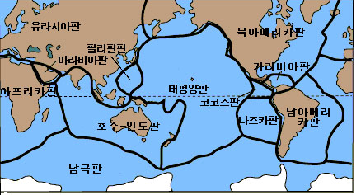
\includegraphics[width=1.0\textwidth]{./fig/plate-001.pdf}
		\end{figure}


\clearpage

1980년대 중반 프랑스의 졸리베 박사는 동해가 만들어진 원인에 대해 앞서 설명한 후배호 확장설과 다른 기발한 아이디어를 떠올렸다. 5천만년 전 인도대륙이 유라시아판에 충돌했기 때문에 일본이 떨어져나갔다는 주장이다. 이 주장을 간단히 이해하기 위해 테니스 공 하나를 떠올려보자. 공을 땅에 대고 한쪽면을 누르면 공은 납작해진다. 이때 누르는 방향과 수직으로 공이 늘어나는 것을 알 수 있다. 이와 같은 원리로 인도대륙이 충돌을 일으키면서 유라시아의 한쪽 귀퉁이에 있는 일본을 옆으로 밀어냈다는 설명이며, 프랑스의 타포니에 박사가 제안한 (인도의 충돌이 약 3천2백만년전 인도차이나 반도의 남진을 야기하였다는) 설을 동해 확장의 기구로까지 확대 적용하였다. 현재 인도판이 한반도에 영향을 미치고 있다는 것은 오늘날 학계의 정설이지만, 2천3백만년전 동해의 확장을 주도하였다는 지질학적 증거가 미약하다. 이러한 이유로 이 설은 후배호 확장설에 가려져 버렸다. 
독자들 중에는 '작은 인도대륙이 거대한 유라시아판에 그렇게 큰 영향을 미칠까?' 라고 미심쩍어 하는 사람도 있을 것이다. 하지만 우리가 보는 작은 인도대륙은 물 위에 보이는 '빙산의 일각'일 뿐이다. 인도판은 유라시아대륙 밑에 엄청난 양의 지각을 밀어넣고 그 한쪽 귀퉁이를 들어 올리고 있는 '얼굴만 작은 장사'다. 인도판은 약 8천만년 전 아프리카 마다가스카르 지괴와 분리된 이래, 1년에 수십cm에 달하는 무서운 속도로 북진했고, 5천만년 전부터 유라시아판에 충돌하기 시작했다(이 시기에 호주판과 결합되었기 때문에 현재는 인도-호주판으로 불린다). 지상 최고의 히말라야산맥이 형성된 것이 바로 이 때문이며, 유라시아와 인도 사이의 바다에서 쌓였던 퇴적물이 3천만년전 급격히 융기하여 고산지대로 되어버린 것이다.

미래의 한반도는 어떤 모습일까?

현재 한국의 동해는 계속 넓어지고 있을까. 그렇지 않다. 지질학적 증거에 따르면 동해가 벌어지는 일이 끝난 것은 대략 1천5백만년 전이었고, 약 5백만년 전부터는 오히려 조금씩 좁혀지고 있다. 
한반도가 속한 유라시아판은 동쪽으로 움직이고 있다. 여기에 정면으로 맞서 동쪽에서 다가오는 것이 태평양판이다. 아래에서는 인도-호주판, 그리고 필리핀해판이 북상하고 있다. 바로 이 4가지 판이 현단계 한반도의 지각변형을 주도하고 있다. 
유라시아판과 태평양판이 서로 가깝게 다가선다는 것은 언젠가는 동해가 다시 닫힐 것을 시사한다. 더욱이 인도-호주판이 북상하면서 유라시아판을 밀어붙여 그 귀퉁이에 있는 한반도와 중국 대륙을 동쪽으로 빠져나가도록 힘을 가하고 있다. 이 힘의 영향으로 중국 대륙내의 북경인근과 만주 지역에는 땅이 벌어져 움푹 꺼진 지구대 지형이 발달하고 있으며, 그 지구대의 동쪽에 위치한 한반도에 동서방향의 압축응력을 발생시키는 것이다. 마치 타포니에 박사의 주장과 같이 인도판이 유라시아판에 충돌해 3천2백만년전 인도차이나 지괴를 옆으로 밀어냈던 것과 같은 원리다. 
하지만 이것은 과거 5천만년 동안의 지괴들의 움직임이 지속된다는 가정하에서 벌어지는 한가지 시나리오일 뿐이다. 언제 이런 일이 벌어질지 정확히 예견하기 어렵다. 일본 국립천문대가 발표한 지구위치정보시스템(GPS)를 분석해보면 최소한 1천만년 후까지 동해가 닫히는 '경향'이 계속되기는 하겠지만, 동해가 완전히 사라지는 일은 그 때까지 벌어지지 않을 것으로 추측된다. 즉 1천만년 후에도 현재 판들 간의 '알력'은 비슷하게 유지될 것이며, 한반도의 모습은 외형상 크게 달라질 것이 없다. 

태평양 속의 해저잠수함

그렇다고 안심할 수만은 없는 상황이다. 1천만년 후에 동아시아에 커다란 영향을 줄 수 있는 무시무시한 복병이 태평양판 안에 존재하기 때문이다. 태평양판의 서측부에는 약 1억2천만년 전 거대한 맨틀이 치솟아 만들어진 돌출부(Shatskiy Rise)가 있다. 한반도보다 조금 큰 규모다. 
문제는 이 돌출부가 연간 약 10cm의 속도로 , 일본의 가미가제 특공대가 2차대전때에 그랬던 것과 반대로, 이번엔 일본을 향해 돌진하고 있다는 점이다. 이들 간의 거리는 불과 약 1천3백km 남짓하는 정도이며, 1천3백만년 후부터 이 거대한 '해저잠수함'이 일본과 부딪히게 된다. 이 돌출부의 밀도는 대륙지각보다 커서, 일본 열도는 물론 한반도를 포함한 동아시아에 일대 지각 변동을 일으킬 것으로 예상된다. 예를 들어 한반도 동해안에는 현재보다 훨씬 강력한 지진이 일어날 것이며, 화산 활동도 곳곳에서 활발하게 전개될 것이다. 또 돌출부의 밀어붙이는 힘 때문에, 표지에서 보여주는 그림처럼, 약 3천만년 후에 동해는 닫혀버릴 가능성이 커진다. 
1천만년 후 한반도에 영향을 미치는 또다른 변수는 인도-호주판이다. 이 판은 현재 동남아시아 군도들을 연간 약 7-10cm 정도의 속도로 힘차게 밀어 붙이고 있다. 그 힘으로 동남아시아 군도가 일본 남단에 도착하는데 걸리는 시간은 약 5천만년 정도 걸릴 것이다. 인도대륙의 북상때문에 작용하는 횡압력의 영향으로, 한반도의 서북쪽의 북경과 만주지방을 잇는 지구대에서는 왕성한 화산작용이 발생하여 땅이 벌어지고, 화산과 깊은 호수도 만들어 질 것이다. 한반도는 중국과 함께 유라시아에서 약간 동쪽으로 밀려나겠지만, 태평양판의 저항에 부딪혀 결국 다시 유라시아판에 귀속될 가능성이 크다. 게다가 현재와 같은 추세대로라면, 남북방향으로 발달된 대서양의 해령의 활동으로 유라시아판은 동진을, 북아메리카판은 서진을 계속하여, 북태평양은 점점 더 좁아지는 반면, 남태평양은 인도양과 대통합이 이루어 진다. 과거 2억년 이상 번성했던 북태평양의 시대가 앞으로 2억년 후면 종말을 맞게된다. 이 때에 남극대륙을 제외한 전세계의 대륙이 하나로 뭉친 초대륙이 형성되고 바야흐로 한반도는 초대륙의 중심부에 위치하게 된다. 
다시 1천만년 후의 세계로 돌아가 보면, 호주는 적도 가까이까지 올라올 것이고, 이때 동남아시아 군도들의 간격이 조금씩 좁혀지면서, 서쪽으로 향하는 적도 해류의 흐름이 차단될 것으로 예상된다. 그렇다면 뜨거운 적도 해류가 역류해 한반도 근해까지 다가올 것이다. 한반도가 현재보다 훨씬 무더운 아열대성 기후로 바뀔 가능성을 보여주는 것이다. 또한 인도-호주판과 태평양판, 동남아시아 군도의 계속되는 압축응력은 뉴기니아섬에 또하나의 히말라야를 탄생하는 방향으로 나아가고 있으며, 히말라야산맥도 지금보다는 좀 더 높아질 것이다. 그러한 지형적 변수는 한반도뿐만 아니라 환태평양 지역의 기후 구도에 일대 변혁을 가져올 것이다. 하지만 지하 자원의 부국이 된다는 좋은 점도 있다. 대륙지각의 충돌은 주변에 엄청난 석유나 금속 자원을 배태하기도 하며, 인도네시아와 중동, 키스피해 주변국들이 그 좋은 예이다.






































% ========================================== chapter ============ 트리즈
\newpage
\chapter{울릉도 독도의 형성}



	% ------------------------------------------ section ------------ 
	\SectionMargin
	\section{울릉도 독도의 형성}
	\null

page 54


% ========================================== chapter ============ 트리즈
\newpage
\chapter{황해의 형성}



	% ------------------------------------------ section ------------ 
	\SectionMargin
	\section{황해의 형성 ( 후빙기 해수면 상승으로 생겨난 황해 )}
	\null



동서 길이 약 700km, 남북 길이 약 1,000km 에 이르는 황해는 한국과 중국에 의해 절반 정도가 닫혀 있고, 평균 수심은 44m, 가장 깊은 곳은 103m로 4,000m를 넘는 동해에 비해 매우 얕다. 그리고 복잡한 지각 변동으로 형성된 동해와 달리 과거 육지였던 곳에 바닷물이 밀려들어오는 매우 단순한 과정을 통해 형성되었다. \\

이러한 차이는 황해의 해저 지형이 쟁반 모양의 완만한 경사를 이루는 분지인데 반해 동해의 해저 지형은 사발 모양의 급경사를 이루는 분지인데 서도 나타난다.\\

황해의 형성 과정을 좀 더 자세히 알아보기 위해서는 먼저 빙하와 해수면 변동의 관계를 이해해야 한다. 지구는 200만 년 전부터 현재에 이르기 까지 대여섯 차례의 빙하 시대를 겪었다. 지구가 추어지면 극지방의 바닷물이 얼어 해수면이 내려가고, 따뜻해지면 빙하가 녹아 해수면이 올라간다. 지금은 빙하가 물러간 후빙기에 해당되며, 현재 남극 대륙을 덮고 있는 빙하가 전부 녹는다면 해수면이 최대 150m 높이까지 상승할 것이라고 한다.\\

마지막 빙하의 최전성기였던 약 1만 8,000년 전에는 바다가 지금의 해안선에서 130~150m 정도 후퇴해 있어 중국, 한국, 일본이 하나의 대륙으로 연결되어 있었다. 그러다가 약 1만 5,000년 전부터 빙하가 물러가면서 해수면이 점차 상승하기 시작해 한국과 중국 사이의 저지대에 바닷물이 밀려들어왔다. 그리고 이러한 과정은 현재의 해수면을 유지하게 된 약 6,000년 전까지 계속되어 황해를 형성했다.\\


% ========================================== chapter ============ 트리즈
\newpage
\chapter{강원도 철원 지질}



	% ------------------------------------------ section ------------ 
	\SectionMargin
	\section{강원도 철원 지질}
	\null



철원 부근에서는 중생대 백악기 말과 신생대 제3기 말 ~ 제4기 사이에 여러 차례 화산활동이 있었다. 현재 철원의 한탄강변에서 발견되는 현무암은 제주도, 울릉도, 백두산 등의 현무암과 궤를 같이하는 것으로 신생대 제4기 말에 있었던 대대적인 화산 활동에 의해 분출 한 것이다.\\

\paragraph{철원의 용암지대}
철원에서는 용암이 백두산이나 한라산처럼 분화구에서 격렬하게 분출하지 않고, 지각의 벌어진 틈을 따라 팥죽이 끊어 넘치듯 조금씩 흘러나왔다. 이 점성이 작은 용암은 저지대의 골짜기를 메우며 퍼져나가 넓은 용암대지를 만들어냈다. 철원의 평야지대는 이렇게 흐른 용암이 굳어져서 평탄 지형이 된 것이다.\\

전곡현무암\\

철원 평야를 덮고 있는 현무암\\


	% ------------------------------------------ section ------------ 
	\SectionMargin
	\section{강원도의 지질}
	\null



주로 【 경기지괴 】와 【 옥천지향사(沃川地向斜) 】에 속하여, 하부는 태백산통(太白山統)으로부터 상부는 신기하성층(新期河成層)까지 한반도 지질계통의 모든 지층이 고르게 분포한다. \\

태백산통은 가장 오래된 지층으로서 주로 편마암으로 구성되어 있고, 화강편마암계(고구려화강암)는 중북부에 주로 분포하여, 분포지는 도 전체의 1/2에 이르며, 곳곳에서 태백산통을 관입한다. \\

조선계(朝鮮系)는 북부 및 남부(영월∼삼척을 잇는 선의 이북)에 비교적 넓게 분포되어 있으며, 양덕통(陽德統)과 대석회암통으로 나뉜다. 양덕통의 하부는 규암, 상부는 셰일 ·점판암 ·천매암으로 구성되어 있고, 양덕통의 상부에 대석회암층이 누층(累層)으로 덮여 있다. \\

평안계(平安系)는 강릉 남부 및 영월 부근에 주로 분포되며, 석탄이 산출되는 지층의 대부분을 포함한다. 본계는 하부에서부터 홍점통(紅店統) ·사동통(寺洞統) ·고방산통(高坊山統) 및 녹암통(綠岩統)으로 구분되며, 특히 사동통의 함탄층에 강릉 ·정선 ·삼척 및 영월탄전 등이 있다. \\

제3기층 및 고기하성층이 국부적으로 분포하고, 고기하성층은 제4기 홍적세에 퇴적된 것으로 보이며, 신기하성층은 현 하천유역에 퇴적된 사력층(砂礫層)으로서 두께는 약 20m 내외이다. 화성암류로는 각 지층에 관입한 화강암이 대부분으로 중부 및 북부에 주로 분포하여 도 전체의 1/3에 해당된다. 철원 부근 한탄강 유역에는 신생대에 분출한 현무암층이 넓게 분포한다. \\




% ========================================== chapter ============ 트리즈
\newpage
\chapter{경상북도 의성 지질}





	% ------------------------------------------ section ------------ 
	\SectionMargin
	\section{경상북도 의성 지질 개설}
	\null



	의성 지역의 기반암을 구성하고 있는 지질은 중생대 쥐라기에 형성된 흑운모 화강암 지대와 
	중생대 백악기에 관입한 화산암류 지대 그리고 중생대 백악기에 형성된 퇴적암류 지대로 구분된다. \\

		\begin{itemize}[itemsep=0.0em]
		\item		【 중생대 쥐라기 】에 형성된 흑운모 화강암 지대
		\item		【 중생대 백악기 】에 관입한 화산암류 지대
		\item		【 중생대 백악기 】에 형성된 퇴적암류 지대
		\end{itemize}


화강암이나 화산암류로 이루어진 지역은 높이가 매우 높은 산지를 이루는 특징을 보이고 있으며, 퇴적암류로 이루어진 지대는 높이가 200~400m 내외의 낮은 구릉성 산지를 이루고 있다.\\

이것은 암석의 단단하고 무른 차이에 따라 나타나는 현상인데, 일반적으로 화성암[화강암, 화산암]에 속하는 암석은 침식과 풍화에 대한 저항력이 강하여 높고 험준한 산지를 형성하는 것이 특징이다. 퇴적암은 사암, 이암, 셰일, 역암 등으로 구성되어 있어 풍화와 침식에 매우 약하다. 이러한 특성 때문에 산지에 풍화가 많이 진행되어 토양층이 두껍게 피복하고 있으며, 산지의 높이가 낮으며 능선이 둥근 형태의 구릉성 산지가 발달한다.


	% ------------------------------------------ section ------------ 
	\SectionMargin
	\section{[중생대 화강암류 지대]}
	\null


의성 지역에서 화강암류는 【 중생대 백악기에 형성된 흑운모 화강암 지대 】와 【 중생대 쥐라기에 형성된 흑운모 화강암 지대 】로 세분된다. 

		\begin{itemize}[itemsep=0.0em]
		\item	[1)] 중생대 백악기의 화강암류 지대\\
				중생대 백악기에 형성된 화강암류 지대는 
				의성군 춘산면 금오리 일대 금오천의 분수계를 이루는 산지가 이에 해당되며, 
				어봉산, 산두봉, 사금령, 화목재가 이에 해당된다. 
				금오천과 사금령을 따라 북서-남동 방향의 단층선이 지나고 있으며, 
				금오천 일대에는 단층 선곡이 발달하고 있는 것을 확인할 수 있다.

		\item	[2)] 중생대 쥐라기의 화강암류 지대\\
				중생대 쥐라기에 형성된 흑운모 화강암 지대는 
				옥산면 금학리의 황학산의 정상부를 중심으로 극히 일부분에 분포하고 있다. 
				이 일대에는 황학산 정상을 중심으로 북서-남동 방향으로 평행을 이루는 
				세 개의 단층선이 발달하고 있다.
		\end{itemize}





	% ------------------------------------------ section ------------ 
	\SectionMargin
	\section{[중생대 화산암류 지대]}
	\null


의성 지역에서 중생대 화산암류로 이루어진 지역은 금성면 수정리 금성산과 비봉산 일대와 가음면 현리리 빙계 계곡, 빙계 온천, 선암산, 북두산, 늑두산 일대이다.

금성산과 비봉산은 산지의 능선이 환상(環狀)의 형태로 연결되어 있으며, 이 두 산지를 잇는 능선을 기준으로 산지의 내측은 산성 화산암으로 이루어져 있으며, 산성 화산암 바깥으로 좁게 띠모양으로 염기성 화산암이 둘러싸고 있다. 화산암의 바깥쪽으로는 퇴적암이 분포하여 지질의 경계가 뚜렷이 구분된다. 금성산 일대는 국내에서 가장 먼저 형성된 화산 지대이며, 화산암과 퇴적암이 경계를 이루는 곳을 따라 기반암이 노출 되어 있는 곳이 많다. 이러한 지점에는 기암괴석이 드러나 있기도 하다.

선암산, 북두산 그리고 복두산 일대는 의성에서 가장 험준한 지역에 해당된다. 지질은 중생대 백악기 유천화산암층군으로 유문암 및 유문 석영 안산암으로 구성되어 있어 침식과 풍화에 대한 저항력이 크다. 따라서 산지 높이가 높으며, 기반암이 드러나 있는 곳이 많아 애추와 같은 지형이 발달하고 있다. 화산암의 분포로 인하여 빙계 온천과 같은 온천도 있다. 또한 화산암은 침식에 대한 저항력이 크므로 하천이 이 지질 구조를 따라 발달할 경우 하상에 기반암이 드러나는 경우가 많다. 빙계 계곡은 유문암 및 유문 석영 안산암으로 이루어진 구간에 쌍계천이 흐르면서 침식하여 드러난 기반암 하상에 위치한다.



	% ------------------------------------------ section ------------ 
	\SectionMargin
	\section{[중생대 퇴적암류 지대]}
	\null


의성의 대부분 지역은 중생대 퇴적암 지대에 해당된다. 독점산, 봉화산, 갈라산, 등운산, 만경산, 장자봉, 왕제산, 봉암산, 곤지봉, 국사봉, 해망산, 응봉산, 천등산, 오동산, 천제봉, 구지봉, 구봉산, 오토산, 생해봉, 수봉실산, 늑두산, 북두산, 복두산 등 산지는 대부분 높이 200~400m 미만의 구릉성 산지인데, 청화산, 갈라산, 다인면의 비봉산 등은 높이가 500~700m 내외로 높다.

퇴적암류도 안평천 부근을 중심으로 동쪽 지역에 해당되는 산지인 봉암산, 곤지봉, 해망산 등은 신동층군에 해당되는 진주층, 문암산층원, 다인층원, 금당리층원으로 구성되어 있으며, 서쪽 지역의 구봉산, 오동산 등은 하양층군에 속하는 점곡층, 후평동층, 일직층 등이 분포하고 있다. 퇴적암으로 구성된 산지는 높이가 낮은 구릉성 산지를 이루는 것이 특징이며, 토심이 깊어 식생의 피복이 좋다.




	\section{[참고문헌]}
	
		\begin{itemize}[itemsep=0.0em]
		\item	『의성 군지』 (의성 군지 편찬 위원회, 1998)
		\item	『1:50,000 지형도』 (국토 지리 정보원, 2005)
		\item	의성군청(http://www.usc.go.kr/)
		\item	한국 지질 자원 연구원 지질 정보 시스템(http://geoinfo.kigam.re.kr/)
		\item	환경부 공간 정보 서비스(http://egis.me.go.kr/egis/home/main.asp/)
		\end{itemize}
	


% ========================================== chapter ============ 트리즈
\newpage
\chapter{추가령 구조곡}




	% ------------------------------------------ section ------------ 
	\SectionMargin
	\section{추가령 구조곡}
	\null

			【 서울 】에서 【 원산 】을 잇는 직선상의 좁은 골짜기로, 
			한반도를 지질적으로 남북으로 양분하는 중요한 경계선이다.\\

			\begin{figure}[h!]
	   		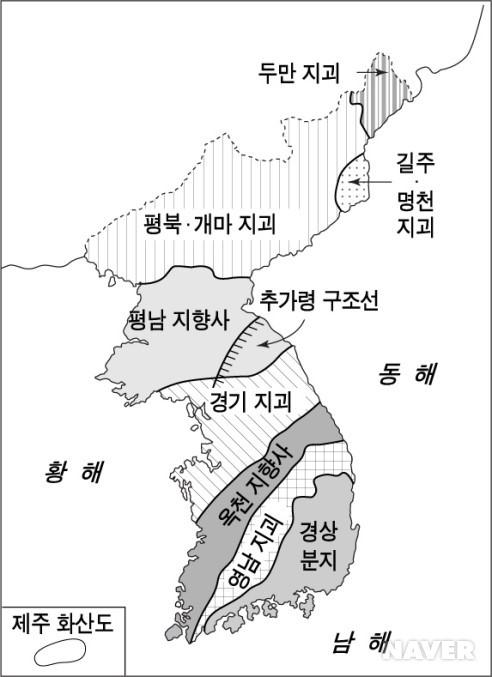
\includegraphics[width=1.0\textwidth,height=1.0\textheight]{./fig/cu-001.jpg}
			\end{figure}
			\clearpage


			철원 일대에 이렇게 광범위하게 용암이 흘러들고 분출한 이유를 알기 위해서는 
			경기도 연천과 강원도 철원 일대를 포괄하는 지체구조인 【 추가령구조곡 】을 먼저 이해 해야 한다. 
			전에는 지구대(단층대)로 불리기도 했던 이 골짜기는 【 서울 】에서 【 원산 】을 잇는 직선상의 좁은 골짜기로, 
			한반도를 지질적으로 남북으로 양분하는 중요한 경계선이다.

			추가령구조곡을 기준으로 북쪽에는 10억년 이상 된 선캄브리아대의 편마암류와 고생대 지층이 우세하다. 
			반면 남쪽에는 이들 지층과 함께 중생대 지층이 넓게 분포하여 남쪽으로 갈수록 형성 연대가 짧아지는 경향이 있다. 

			또한 북쪽의 산맥들은 대체로 북동동~남서서의 랴오둥 방향으로 뻗어 있으나 남쪽의 산맥들은 북동~남서의 중국방향으로 뻗어 있다.

			단층이란 지각에 생긴 틈을 경계로 양쪽 지괴가 상대적으로 어긋난 것이다. 
			한때 추가령구조곡은 평행한 두 단층 사이에 긴 띠 모양의 지층이 내려앉아 형성된 지구대로 생각되었다. 
			그러나 여러 차례의 지질 조사 결과, 단층들 사이에서 약한 띠를 이루던 화강암체가 추가령(586)을 분수계로 
			남대천과 임진강에 의해 차별침식을 받아 만들어진 단층선곡(斷層線谷)인 것으로 밝혀졌다. 
			이런 단층선을 따라 용암이 쉽게 분출할 수 있었기 때문에 철원평야와 같은 대규모의 용암대지가 형성된 것이다.

	\SectionMargin
	\section{추가령 구조곡 정의}

			광주산맥과 마식령산맥 사이 대략 서울∼원산을 잇는 북북동∼남남서 방향의 단층선곡(斷層線谷).



	\SectionMargin
	\section{추가령 구조곡  명칭 유래}

			추가령이라는 지명은 이 열곡의 중북부에 위치한 북한의 강원고 고산군 삼방리와 세포군 세포리 사이의 
			용암대지에 개석된 단애에서 기원한 것으로 이 지역은 분수계는 아니지만 일반인들에게 고개로 인식되고 있다.




	\SectionMargin
	\section{추가령 구조곡  형성 및 변천}

			과거에는 이 구조곡의 방향과 나란히 다수의 정단층이 존재하고 있는 것을 근거로 
			단층에 의해서 형성되는 지구대와 동일시하여 이 구조골짜기를 【 지구대 】
			\footnote{지구대 [地溝帶]\\ 단층 운동의 결과, 단층 사이에 함몰된 낮은 지대가 길게 연속적으로 나타나는 지형을 지구대라고 한다. 지구대는 일반적으로 평탄한 특징을 가지고 있기 때문에 지구대를 따라 하천이 흐르며, 보통 교통로로 많이 이용된다. 우리나라에는 신생대 제3기 때의 지각 운동으로 형성된 길주 · 명천 지구대와 형산강 지구대가 있다. 길주 · 명천 지구대를 따라 함경선, 형산강 지구대를 따라 동해 남부선 철도가 지나고 있다(Basic 고교생을 위한 지리 용어사전, 2002.2.5, (주)신원문화사)} 
			라 하였다.

그러나 그 뒤에 이루어진 조사에 의하면 이 지대가 저지대로 된 것은 중국방향의 단층선에 연하여 화강암이 관입(貫入)하고, 이 화강암이 그 양측의 접촉변질(接觸變質)된 변성암을 주로 하는 고기암층에 비하여 침식에 대한 저항력이 약하기 때문에 차별침식(差別浸蝕)을 받은 결과로 지구대와 같은 지형이 형성된 것이다. 그 밖에 지구대로 인정될만한 단층운동의 증거가 없다는 것이 밝혀졌다. 

신생대 말기에 해당하는 제4기에 평강에서 남서쪽으로 3km에 위치한 오리산(454m)을 중심으로 열하 분출한 현무암이 【 구조선 】\footnote{지질구조선 [ 地質構造線, tectolineament ]지층이나, 좁게는 기반암석, 더 좁게는 독립된 암체 등에 나타나는 선구조로 주로 내적인 영력과 같은 지각운동에 의해서 형성되는 것이다. 구조선이라고도 한다. 형태는 지각에 틈새가 벌어진 형태로 이 틈새가 길게 연장되어 선적으로 발달하여 있다. 소규모의 것은 절리(節理, joint)로 그 규모는 수 ㎝에서부터 나타나며, 대규모는 대단층선으로 수천 ㎞에 이르는 것도 있다. 지질구조선이 발달한 부분은 지형적인 측면에서는 풍화와 침식에 약한 부분이 된다. 따라서 길게 연장되어 있는 지질구조선을 따라서 지표의 개석이 이루어지면 산지와 곡지의 기복이 뚜렷하게 발달하게 되어 결국 산맥이나 구조곡과 같은 지형의 근원이 되기도 한다} 을 따라 분출되어 이른바 철원·평강 용암대지를 형성하였으며, 이 용암은 열곡을 따라 북쪽으로는 남대천을 따라 북한의 강원도 고산군 북부일대까지, 남쪽으로는 한탄강과 임진강을 따라 경기도 파주시 파평면 일대까지 흘러내렸다.

이 용암 분출로 인하여 이 【 구조곡 】\footnote{구조곡 [ 構造谷 ]\\ 지질 구조가 상이한 두 지괴의 경계선 또는 단층선을 구조선이라고 하는데, 이 구조선은 형성된 지각의 지질 구조를 반영한다. 단층 운동으로 지각이 갈라진 구조선을 따라 오랫동안 차별 침식이 이루어지고 주변 지역보다 깊게 파이면 좁고 긴 골짜기인 구조곡이 형성된다. 우리나라의 대표적인 구조곡은 【 추가령 구조곡 】을 들 수 있는데, 이 지역은 편마암 지역 사이에 화강암이 관입된 후 차별 침식으로 골짜기가 형성된 것이다. 이 구조곡을 따라 경원선 철도가 지나간다.(Basic 고교생을 위한 지리 용어사전, 2002.2.5, (주)신원문화사)}을 따라 북동쪽으로 흐르는 안변 남대천과 임진강의 지류 평안천(平安川)간의 하천쟁탈현상이 있었다. 즉, 남대천은 옛 분수령으로부터 남으로 21㎞ 정도 연장되었는데, 이는 남대천이 옛 분수령 이남의 평안천 상류부를 쟁탈한 결과이다. 평안천의 상류부를 쟁취한 남대천은 이 구조선의 북쪽 부분을 따라서 거의 직선상으로 흐르고, 하곡을 깊게 하각(下刻)하여 석왕사곡(釋王寺谷)ㆍ삼방협곡(三防峽谷) 등 깊은 협곡을 만들고 있다.

특히, 삼방협곡에는 지형적 이점을 이용하여 과거 통행인을 검문하는 3개소의 관방(關防)이 설치되어 있었고, 삼방협곡이라는 이름도 여기서 유래된 것이다.




	\SectionMargin
	\section{추가령 구조곡  현황}

			이 구조선은 우리나라의 지체구조(地體構造)를 남북으로 이등분하는 경계선이 되어 
			그 【 북쪽 】은 【 랴오둥 방향 】의 구조가 탁월하고, 【 남쪽 】은 【 중국방향 】의 구조가 탁월하다. 

			이 지역은 안변 남대천, 북한강, 임진강, 한탄강 유역이 접하는 복잡한 분수계 혼란 지역으로 
			분수계의 핵심은 평강의 오리산이며 이를 중심으로 4개의 분수계가 갈라지는 분수점 기능을 하고 있다.



	\SectionMargin
	\section{추가령 구조곡 참고문헌}
	
		\begin{itemize}[itemsep=0.0em]
		\item	『한국지리지(韓國地理志) -강원편(江原篇)』(국토지리정보원, 2006)

		\item	「추가령 열곡 연천 고호소층의 퇴적물 기원지 분석」
				(이민부ㆍ이광률ㆍ김남신, 『대한지리학회지(大韓地理學會誌) 42(1)』, 2007)

		\item	「추가령 열곡의 철원-평강 용암대지 형성에 따른 하계망 혼란과 재편성」
				(이민부ㆍ이광률ㆍ김남신, 『대한지리학회지(大韓地理學會誌) 39(6)』, 2004)
		\end{itemize}






% ========================================== chapter ============================ 
%
%
%
% ========================================== chapter ============================ 
\newpage
\chapter{한국지체구조도}




	% ------------------------------------------ section ------------ 
	\SectionMargin
	\section{한국지체 구조도}

		\clearpage
		\includegraphics[scale=0.9,  width=1.0\textwidth]{./fig/fig_001.pdf}

		\clearpage
		\includepdf[pages=-, scale=0.9, frame=true, landscape=false]{./fig/fig_002.pdf}	

		\clearpage
		\includepdf[pages=-, scale=0.9, frame=true, landscape=false]{./fig/fig_003.pdf}	


	% ------------------------------------------ section ------------ 
	\SectionMargin
	\section{한반도의 지질과 지체구조}
	\null

		\includegraphics[width=0.60\textwidth]{./fig/fig_003.pdf}


한반도의 지체구조는 땅덩어리가 언제 어떻게 만들어졌나 하는 것에 초점을 맞춰서 이해하세요~

한반도는 시원생대때 이미 어느 정도 한반도의 형상을 갖추고 있습니다. 우리나라가 오래된 땅이라는 증거지요. 고생대와 중생대 신생대를 거쳐 한반도의 형상이 완성되었는데, 이를 순서대로 나누어서 생각해 봅시다. 


		\includegraphics[width=1.00\textwidth]{./fig/fig_004.pdf}


우리나라는 위 순서대로 만들어졌습니다. 

시원생대 이미 많이 만들어 졌고, 고생대, 중생대, 신생대에 와서는 일부 지역만 만들어졌네요. 

		\begin{itemize}[itemsep=0.0em]
		\item	[①] 시원생대 (평북․개마지괴,경기지괴,영남지괴) : 가장 오래된 안정지괴
		\item	[②] 고생대 (평남지향사,옥천지향사) : 해성층, 조선계에는 석회암, 평안계에는 무연탄매장
		\item	[③] 중생대 (경상분지) : 육성층 → 수평 퇴적층 발달, 공룡발자국 화석발견
		\item	[④] 신생대 (두만지괴,길주 명천 지괴) : 분포 범위가 좁으며 제3기층 일부에 갈탄매장
		\end{itemize}	




	% ------------------------------------------ section ------------ 
	\SectionMargin
	\section{한반도의 지체구조}
	\null


		지체 구조는 서로 다른 성질을 가진 땅 덩어리의 구조이다. 
		한반도 역시 다양한 지형 형성 작용이 있었기 때문에 서로 다른 덩어리들로 나눌 수 있다.

		\subsection{지괴 ( 땅덩어리 )}
				▶평북⋅개마지괴, 경기지괴, 영남지괴: \\
				지괴는 말 그대로 주변과 구분되는 땅덩어리(landmass)를 의미해. \\
				地 땅 지 / 塊 덩어리 괴 금괴\\
				이들 지역은 오랫동안 안정된 상태로 계속 육지로 노출되어 있었던 곳이야.
				그런 만큼 지질의 측면에서 봐도 주로 선캄브리아기의 변성암으로 구성되어 있지.
				
		\subsection{지향사}
				▶평남지향사, 옥천지향사 : \\
				지향사는 땅의 방향이 기울어 졌다는 뜻이지? \\
				이는 지각 일부가 기울어지면서 침강한 지역에 두꺼운 퇴적물이 쌓인 곳을 말해. \\
				地 땅 지 지각 / 向 방향 향 /斜 기울어질 사 경사

				고생대 때 한반도가 침강해 한반도의 지괴들 사이의 저지대는 지향사가 되었어.
				여기가 중요! 
				그런데 고생대 중기까지는 바다에 잠겨 있다가 
				중기 이후에는 조륙 운동으로 다소 융기하여 넓은 호수의 지향사였다는 거야!
				
				그래서 고생대 전기에는 바다 속에서 만들어진 해성(海成)층인 【 조선계 지층 】이 나타나는데 
				이때의 대표적인 퇴적암이 석회암이야.
				고생대 후기에는 넓은 호수에 퇴적된 육성(陸成)층인  【 평안계 지층 】이 만들어졌는데
				그 안에 무연탄이 매장되어 있지.
				그래서 고생대 지층을 살펴보면 
				같은 지역의 하부 지층에는 석회암이, 상부 지층에는 무연탄이 묻혀 있는 거란다.
				
				지향사의 위치와 석회암 및 무연탄의 분포 지역이 일치한 다는 것을 지도로 확인할 수 있어.
				
				
				
				\textbf{지향사 地向斜 geosyncline}
				
				지(地) : 땅 지 | 흙 토(土) + [어조사 야(也)→지]\\
				향(向) : 향할 향 | 입 구(口) + 집 면(宀)\\
				사(斜) : 비낄 사 | 말 두(斗) + [나 여(余)→사]\\
				땅(地)을 향(向)해 생긴 경사(斜)\\
				지향사(地向斜)는, 
				지층이 수천 미터 이상 두껍게 퇴적된 후, 조산운동을 받아 경사를 이룬 퇴적 분지를 말합니다.\\				
막대한 양의 퇴적물이 쌓이는 지각 내의 선형 함몰대.\\
지향사 내에 수천에서 수만m 두께의 퇴적물이 채워지면서 퇴적의 마지막 단계에서는 습곡·붕괴·단층 작용이 수반된다. 결정질 화강암의 관입과 함몰대의 축을 따라 일어난 광역적 융기에 의해 특정 지향사의 형성은 완료되고, 습곡산맥으로 변환된다. \\
지향사의 개념은 1859년 미국의 지질학자 제임스 홀에 의해 소개되었고, 이것은 조산운동 개념의 기초가 되었다. 오늘날에는 한 지향사가 2구역으로 분할되어 있다는 생각이 세계의 많은 산맥계의 암층 내에서 확인되고 있다. 잡사암(泥質·基質의 암편이 많이 포함된 사암)·처트 및 심해 퇴적작용의 과정을 반영하는 다양한 퇴적암들과 함께 존재하는 두꺼운 화산 층서는 지향사 외곽의 심해 부분인 완지향사에서 퇴적된 것이다. 한편 석회암과 분급이 잘 된 석영질 사암의 존재는, 이것이 천해에서 형성되었다는 증거로 생각되며 이런 암석들은 차지향사라 불리는 지향사의 안쪽에서 만들어진다. 한 지형사의 분할 외에도 몇 가지 유형의 유동대가 인지되고 명명되었는데, 이중에서 좀더 흔한 형태로는 하나 이상의 급경사 단층에 의해 둘러싸이고 퇴적물이 퇴적되는 침강한 지괴인 타프로 지향사와 대륙 주변부에서 해안평원으로 변환하는 심해 지향사인 파랄리아 지향사가 있다.\\
				
				
		
		\subsection{분지}
		
			\subsubsection{경상 분지}
				경상도 지역에 있었던 퇴적 분지를 말해. \\
				이를 구성하는 지층은 ‘경상계 지층’이라 하지.
				중생대 말에 경상도 지역은 넓은 호수였고 여기에 두꺼운 육성층이 형성되었지.
				이 때 여기에 공룡이 엄청 살았대나봐. 
				그래서 경상계 지층에는 공룡 화석이나 발자국이 많이 발견되지.\\
				
			\subsubsection{두만 지괴, 길주⋅명천 지괴}
				이들 지괴는 신생대 제3기에 만들어진 지층으로  분포 범위가 좁아. \\
				갈탄이 묻혀있어 북부 지방에서는 에너지 자원으로 쓰이지.\\
				
				▶그러면 신생대 제 4기는?
				퇴적층으로 존재하는데
				하천이나 해안 주변의 충적층이 이에 해당돼.\\
				


		\newpage
		\includepdf[pages=-, scale=0.9, frame=true, landscape=false]{./fig/fig_005.pdf}	

		\newpage
		\includepdf[pages=-, scale=0.9, frame=true, landscape=false]{./fig/fig_006.pdf}	




한반도는 탄생 이래 침강과 융기를 반복하는 조륙(造陸)운동을 거치며 지속적으로 침식되었다. \\

		\subsection{고생대 초}
				약 5억 7,000만 년 전 고생대 초에 이르러 
				선캄브리아대 육괴들 사이의 저지대가 얕은 바다에 잠기면서 
				선캄브리아대 기반암위로 퇴적층이 형성되었다. 
				이후 중생대 초까지 바다로 덮여 있는 동안 두꺼운 퇴적층이 쌓였는데, 
				평남지향사와 옥천지향사가 이에 속한다.
				
				바다 환경이 지속되는 동안 삼엽충을 비록한 완족류와 두족류 등의 초기 생명체가 번성했으며, 
				바다 밑으로 조류와 산호 등의 침전물이 쌓여 조선누층군이 형성되었다. 
				평안남도 남부와 강원도 남부 일대에 분포하는 석회암층은 바로 이때 만들어진 것이다. \\

【 고생대 초 】에 한반도는 지금의 위치가 아니라 적도 이남 10 부근에 있다가 점차 북상하여 【 중생대 트라이아스기 】에 북위 25에 도달했으며, 약 2억 년 전 【 쥐라기 】에 이르러 지금의 38 부근에 도달했다.\\


		\subsection{고생대 말}
				약 2억 9,000만년 전 페름기(고생대 말)로 접어들면서 
				바다가 후퇴하여 바다 환경이 육지 환경으로 바뀌었다. 
				이때 거대한 늪지대가 형성되었는데, 
				석탄기에 번성했던 양치 식물과 석송류가 울창한 숲을 이루었다. 
				이후 두껍게 퇴적된 삼림대가 지하 깊은 곳으로 함몰되고, 
				이어 열과 압력에 의해 탄화하여 조선누층군 위로 평안누층군을 형성했다. 
				평안남도와 강원도 일대의 탄전지대에 분포하는 석탄은 모두 이 시기에 만들어진 것이다.\\

		\subsection{중생대}
특별한 지각 변동 없이 고생대까지 안정을 유지해오던 한반도 땅덩어리는 중생대에 이르러 엄청난 지각변동의 소용돌이에 휩싸이게 된다. 여러 차례의 화산 활동을 동반한 습곡과 단층 작용의 영향으로 지각이 갈라지고, 지층의 내려앉거나 올라가거나 휘어지는 등 일대 격변을 겪었다. \\

		\subsection{중생대 초 트라이아스기}

				약 2억 3,000만년 전 중생대 초 트라이아스기에는 
				【 송림변동 】이라는 거대한 조산 운동이 북한 지역에 집중적으로 일어났다. 
				이로 인해 고생대 지층인 평남지향사가 들어 올려 졌으며 지층이 심한 습곡을 받았다.\\

		\subsection{중생대  쥐라기}
				약 1억 4,000만 년 전 쥐라기 말로 접어들면서 
				한반도 지질 역사상 가장 격렬했던 지각 변동이 【 대보조산운동 】이 한반도 전역에서 일어났다. 
				그 결과 기존의 한반도 지질 구조에 엄청난 변화가 일어났고, 
				지하 깊은 곳에서 대규모의 마그마가 관입하여 대보화강암이 형성되었다. 
				우리나라의 대표적인 화강암 산지인 금강산, 설악산, 계룡산, 북한산, 관악산 등지에 
				가득한 암석들은 모두 이때 형성된 것이다. 
				송림변동과 대보조산운동의 영향으로 한반도에는 땅의 곳곳이 갈라지는 균열선, 
				즉 구조선이 생겨났고, 
				이 구조선을 따라 오랫동안 침식이 이루어져 오늘날의 산맥과 같은 모양새가 만들어 졌다.



		\subsection{중생대 말 백악기}

				한반도에 공룡 시대가 전개 되었던 약 9,000만 년 전 백악기 말로 접어들면서, 
				영남 지방을 중심으로 【 불국사운동 】이 일어나 
				화산 분출과 함께 단층, 습곡 작용으로 지층이 교란되었으며, 불국사화강암이 관입했다. 
				월악산, 속리산, 월출산, 토함산, 금정산 등지의 화강암 덩어리들은 이때 만들어진 것이다. 
				또한 곳곳에 지반이 내려앉아 거대한 분지가 생겨났고, 
				이곳으로 물이 흘러들어 호수가 만들어졌다. 
				이후 오랫동안 호수 바닥에 퇴적물이 쌓여 두꺼운 경상계 퇴적층이 형성되었는데 
				고성 덕명리, 해남 우항리, 화성 시화호 등지에서 발견되는 공룡 알 화석은 
				모두 이 퇴적층에 남은 것이다.




		\subsection{신생대 제3기 중기 ; 동해의 생성 및  경동성요곡운동 }

				불국사운동을 겪은 후 한반도에는 큰 지각 변동 없이 오랫동안 침식이 일어났다. 
				그러나 약 2,300만 년 전 신생대 제3기 중기 마이오세에 이르러 
				한반도 땅덩어리는 다시 크게 요동쳤다. 
				일본이 한반도에서 떨어져 나가면서 그 사이에 동해가 생겨났고, 
				동해의 해저 지각이 확장하면서 한반도 땅 덩어리를 밀어붙여 한반도가 위로 솟아올랐다. 
				이때 융기축이 동쪽에 치우친 요곡 운동이 일어나 낭림산맥, 함경산맥, 태백산맥 등이 
				높게 솟아 올랐고, 이러한 융기는 지금도 계속되고 있다.\\

				한반도는 중생대에는 바다의 영향을 거의 받지 않았다. 
				하지만 신생대에 이르러 동해안 몇몇 곳이 바다에 잠기며 퇴적층이 형성되었다. 
				두만지괴, 길주명천지괴, 포항분지 일대가 
				그 당시에 형성된 퇴적층으로, 석유와 천연가스의 매장 가능성이 높아 주목을 받고 있다. \\



		\subsection{신생대 제3기 말에서 제4기 초 ( 화산 활동 )}

				신생대 제3기 말에서 제4기 초인 약 200만 년 전을 전후하여 
				전국 곳곳에서 일어난 화산 활동으로 백두산, 제주도, 울릉도, 독도가 생겨났고 
				개마고원, 철원~평강 지역, 신계~곡산 지역에 거대한 용암지대가 형성되었다.\\
				
				중생대 이후 구조선을 따라 계속적으로 일어난 침식 작용으로 
				한반도의 산맥은 더욱 뚜렷한 골격을 갖춰갔다. 
				

		\subsection{신생대 제4기}

				제4기로 접어들면서 한반도는 여러 차례【  빙하에 의한 해수면의 승강 운동 】을 겪었는데, 
				그 결과 동해안에는 해안단구가 집중적으로 발달했으며, 
				황남해안에 리아스식 해안이 형성되었다.\\


		\newpage
		\includepdf[pages=-, scale=0.9, frame=true, landscape=false]{./fig/fig_007.pdf}	





% ========================================== chapter ============================
%
%
%
% ========================================== chapter ============================
	\newpage
	\chapter{누층군}

	% ------------------------------------------ section ------------ 
	\SectionMargin
	\section{경상 누층군}
	\null

경상누층군은 주로 강유역의 범람원에서 만들어진 퇴적 지층으로, 형성 시기는 지금부터 약 1억1000만면 전의 중생대 전기로 확인되었다.\\

우리나라 중생대 백악기를 대표하는 지층이다.\\

【 경상계 】라고 부르며, 선캄브리아 시대부터 중생대 초에 형성된 지층을 부정합\footnote{퇴적이 중단되거나 먼저 퇴적된 층의 일부를 잃어버린 상태에서 다시 퇴적이 되어 시간적인 공백이 있는 지층부정합에서 가장 중요한 것은 층과 층 사이에 시간적인 공백의 유무이다. 만약 두 개의 서로 다른 층 사이에 시간적인 공백이 있다면 그것은 부정합이 된다. 부정합이 만들어 지기 위해서는 퇴적이 중단되거나 먼저 퇴적된 층의 일부분이 사라져야만 한다. 그 후 다시 퇴적이 일어나는데 이때 퇴적이 중단된 면이나 침식된 면을 부정합면이라고 한다[네이버 지식백과] 부정합 [unconformity, 不整合] (두산백과)} 으로 덮고 있다.\\

경상누층군은 크게 두층으로 되어 있다. \\
아래에 있는 층은 지질학 용어로 【 낙동통 】이라 부른다. 주로 붉은색 셰일이나 사암 또는 역암이 교대로 쌓여 있고 사이에 간혹 무연탄층이 발달해 있다. 두께는 약 4000미터에 이른다. 
위에 있는 층은 【 신라통 】으로 부르고 역시 붉은색 셰일이나 사암 등으로 되어 있으며, 두께는 약 3600미터에 이른다. 신라통은 낙동통을 【 평행부정합 】으로 덮고 있다.

		\newpage
	% -------------------------------------- page -------------------
		\subsection{셰일 [ shale ] }


		운반작용으로 생성되는 퇴적암 중 입자의 크기가 63㎛(마이크로미터)보다 작고, 층과 평행하게 벗겨지는 암석.\\

		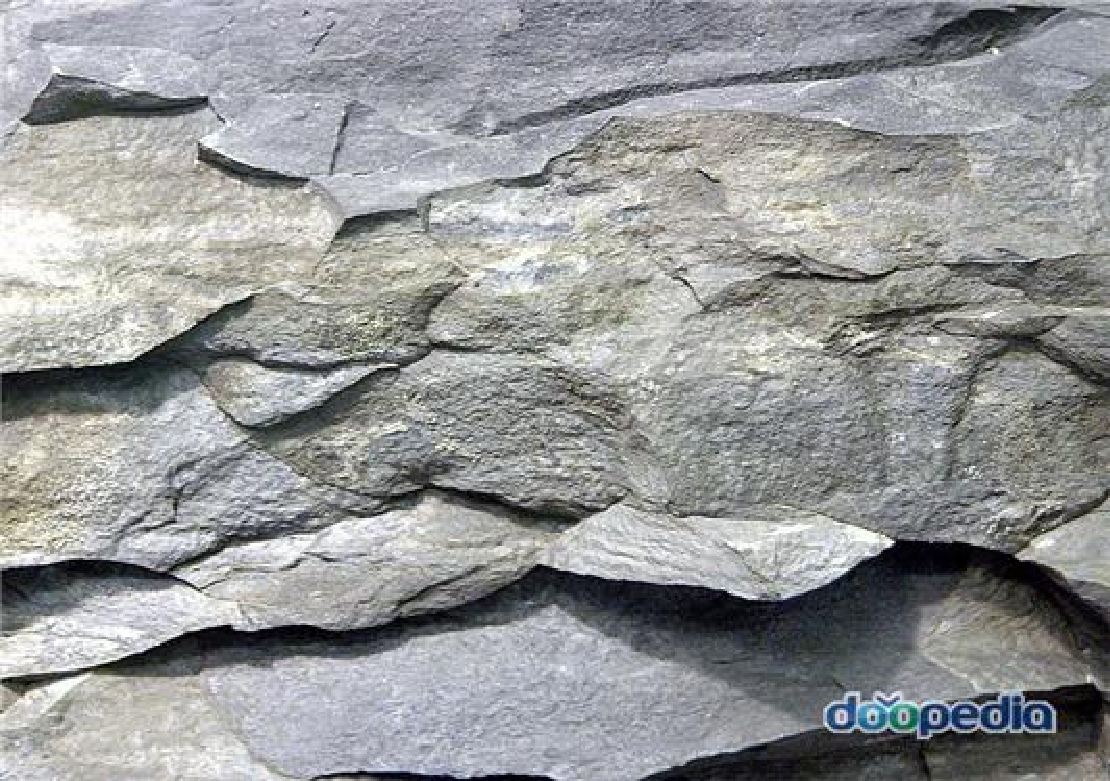
\includegraphics[scale=0.9,  width=1.0\textwidth]{./fig/fig__101.pdf}


		입자의 크기가 63㎛보다 작은 세립질의 암석으로, 전형적 층상구조를 보여 쪼개짐이 나타난다. 
		성층면(成層面)을 따라 평행하게 얇은 층으로 쪼개지는 성질을 가지는데, 
		이것은 입자의 크기가 다르거나 구성광물의 색이 다를 경우 나타난다. 
		흰 쌀과 검은 쌀을 층층이 쌓은 것을 생각하면 된다. 붉은색, 녹색, 검은색, 회색 등 여러 색이 나타난다.
		[네이버 지식백과] 셰일 [shale] (두산백과)


	% ------------------------------------------ section ------------ 
	\SectionMargin
	\section{조선 누층군}
	\null

		Choseon supergroup, 朝鮮累層群\\

		평안남도·강원도 및 경상북도 북부에 넓게 분포하며, 
		그밖의 지역에도 산재되어 분포하는 고생대 전기에 퇴적된 지층을 말한다





	% ------------------------------------------ section ------------ 
	\SectionMargin
	\section{평안 누층군}
	\null

		\setlength{\fboxsep}{12pt}
		\begin{boxedminipage}[c]{1.0\linewidth}
			평양특별시 부근과 평안남도 덕천시,\\
			강원도 삼척군·영월군·정선군, \\
			충청북도 단양군에 분포된 석탄기에서 트라이아스기초에 걸친 퇴적암 누층군.
		\end{boxedminipage} \null



		고생대 전기의 퇴적암층을 조선누층군 석회암\\
		고생대 후기의 퇴적암층을 평안누층군 사질 퇴적암 이라 한다.\\

		평안계라고 불려온 지층이다. 
		'평안계'는 처음 평양 부근에서 홍점층(紅店層)·사동층(寺洞層)·고방산층(高坊山層)·녹암층(綠岩層)의 4개층으로 구분되었는데, 
		1940년에 강원도 삼척탄전에서 암질이 비슷하고 화석 내용도 비슷한 지층이 발견되어 위의 지층명이 그대로 사용되었다. 

		\newpage
	% -------------------------------------- page -------------------
		\subsection{삼척탄전}
		
		삼척탄전의 평안누층군은 최근(1969) 암질과 화석을 기준으로 만항층(晩項層:대체로 홍점층에 해당함)·금천층(錦川層:대체로 하부 사동층에 해당함)·장성층(長省層:대체로 상부 사동층에 해당함)·함백산층(咸白山層:고방산층의 하부)·도사곡층(道士谷層:고방산층의 중부)·고한층(古汗層:고방산층 상부)·동고층(東古層:녹암층 하부에 해당)으로 나뉜다.\\

만항층은 홍색 또는 담녹색을 띤 셰일·사암·역암으로 구성되어 있으며, 흰색의 석회암을 협재한 석탄기 중엽의 지층으로 최하부의 암회색 셰일에서는 식물화석이 발견된다. 석회암에서는 바다화석이 발견되며, 방추충은 식물화석과 함께 지층의 퇴적이 석탄기 중엽(모스코비안)에 이루어졌음을 알게 한다.\\

 금천층은 회색 또는 암회색의 사암·셰일·석회암으로 되어 있으며, 석회암에서는 모스코비안 후기의 방추충이 발견된다. 만항층의 일부는 육성층이지만 대부분은 해성층이고 금천층도 해성층이다. 금천층을 덮는 장성층은 회색 또는 암회색의 셰일, 사암으로 되어 있으며, 무연탄층을 2~4매 협재하고 석회암은 협재하지 않는다. 장성층은 4개의 윤회층(輪廻層)으로 되어 있으며 3번째 윤회층에 협재된 무연탄층이 가장 두껍다. 이 석탄층의 상반 셰일층에는 많은 종의 페름기 식물화석이 포함되어 있다. \\
 
 함백산층은 주로 백색사암(규화됨)으로 되어 있으며 암회색 셰일을 수매 협재한다. 여기서는 식물화석이 거의 발견되지 않는다. 도사곡층은 주로 자색·황색·홍색·담녹색의 사암으로 되어 있으며, 간간이 셰일을 협재하는데 이 셰일에서는 드물게 페름기의 식물화석이 발견된다. 고한층은 회색 셰일을 주로 한 지층이며 식물화석을 거의 포함하지 않는다. 동고층은 담녹색의 사암·셰일 및 적색의 사암으로 구성되어 있다.\\

금천층과 장성층 사이는 준정합 관계에 있는 것으로 보인다. \\
\null \hfill 鄭昌熙 글

		\newpage
	% -------------------------------------- page -------------------
		\subsection{영월탄전}

영월탄전의 평안누층군은 아래에서 위로 다음과 같이 구분되었다. 즉 요봉층(要峰層:최하부를 제외하면 만항층에 대비됨)·판교층(板橋層:대체로 금천층에 해당함)·밤치층(이는 삼척탄전에서 발견되지 않은 페름기 초엽의 해성층임)·미탄층(美灘層:대체로 장성층에 대비됨)으로 구분되며, 고방산층에 해당하는 지층은 지표에 노출되어 있지 않은데 이는 미탄층의 상부가 마차리 역단층으로 잘려 있기 때문이다. 영월탄전에서는 판교층(석탄기 모스코비안 후반기의 지층) 위에 밤치층(페름기 사크마리안의 지층)이 놓이는데, 이러한 사실은 시대를 명시하는 방추충에 의해 단일 석회암층 중부에서 증명되었으므로, 이 경계가 1,000만 년의 시간 간격을 의미하는 준정합임이 분명하다. 즉 이 준정합은 석탄기 말엽의 우랄리안과 페름기초의 앗셀리안을 대표할 지층의 결여를 의미한다. 고한층과 동고층도 평행부정합 관계에 있다. 고한층은 트라이아스기의 것으로 보이나 아직 화석에 의한 증거는 없다. 평창탄전에 넓게 분포된 녹암층(하부는 동고층에 해당)은 두께가 2,400㎜에 달한다.\\
\null \hfill 鄭昌熙 글

% ========================================== chapter ============================ 분지
%
%
%
% ========================================== chapter ============================ 분지
	\newpage
	\chapter{분지}



	% ------------------------------------------ section ------------ 
	\SectionMargin
	\section{경상 분지}
	\null





\subsection*{1. 경상분지}

대규모의 신장력이 작용하면, 정단층을 동반한 거대분지가 만들어 질 수 있다. 그 예가 바로 우리나라의 경상분지이다. 이 경상분지는 중생대 말기에 만들어진 것으로, 호수 환경에 많은 양의 육상 퇴적물이 쌓여 퇴적암이 만들어졌다.




\subsection*{2. 경상분지}

한반도는 【 \textbf{고생대} 】 이래로 큰 지각 변동 없이 오랜 기간 침식을 받아 준평원에 가까운 평탄 지형을 유지해왔다. 
그러나 【 중생대 쥐라기 】에 접어들면서 전국에 걸쳐 【 대보조산운동 】이 일어나 지각의 일부가 오르내리면서 지층이 휘어졌고 격렬한 화산과 지진 활동으로 지반이 크게 요동치는 불의 시대가 도래했다.\\

이어 【 중생대 백악기 】에 전국적으로 또 한 번의 대대적인 지각변동인 【 불국사운동 】이 일어나 곳곳에 수십~수백 km 규모의 분지형 저지대가 형성되었다. 저지대인 분지로 물이 흘러들어 점차 커다란 호수가 만들어졌고, 호수 주변으로는 많은 못과 늪지대가 생겨났다.\\

경상남도 고성과 진주, 경상북도 의성을 비롯한 경상도 일대와 전라남도 해남과 함평, 능주, 전라북도 진안과 부안, 충청남도 공주, 충청북도 음성, 강원도 통리 등 중생대 백악기 퇴적층이 분포하는 지역은 모두 당시 분지였던 곳으로, 분지에 물이 고여 생겨난 호수에 퇴적물이 쌓여 형성되었다.\\

당시 경상도 일대의 저지대를 경상분지라 하며, 그 분지로 물이 들어와 생겨난 호수를 【 경상호수 】라 한다. 경상호수는 경상도 전역은 물론 대한 해협과 일본 본토까지 아우르는 거대한 호수였던 것으로 알려져 있다. 공룡 발자국이 나타나는 고성 덕명리 해안은 경상호수에 쌓인 퇴적층인 경상 누층군의 일부이다. 경상 누층군의 두께가 10km 정도라 하니 얼마나 큰 규모의 호수에서 얼마나 오랜 기간 쌓였는지 가늠할 수조차 없을 정도이다.\\





% ========================================== chapter ============ 트리즈
\newpage
\chapter{산계}



	% ------------------------------------------ section ------------ 
	\SectionMargin
	\section{1. 산계 개요}
	\null


	대륙적 규모에서 발달하는 최대급의 산지 계통. 대개 둘 이상의 산맥이 서로 밀접한 관계를 가지고 한 계통을 이룬다.

	히말라야 산계\\	
	태백 산계. \\

	【 산계 】는 산맥들의 모임을 말하며 산맥에 따라서는 큰 명칭 속에 작은 산맥을 
	경험적으로 칭하여 포함하기도 한다.\\

	즉, 우리 나라 태백산맥 속의 설악산맥이라는 경험적 소구분을 하기도 한다. 
	산맥은 지질구조, 조산운동의 과정과 외인적인 강수량의 다과에 따른 침식·풍화 작용 등에 따라 서로 상관하여 이루어지며, 
	대체로 지질구조의 축(軸)과 일치되는 경우가 많다. \\


	% ------------------------------------------ section ------------ 
	\SectionMargin
	\section{2. 우리나라 산계의 구분}
	\null


		우리 나라의 산맥은 지질구조와 산맥방향에 따라 【 중국방향산계 】와 【 요동방향산계 】 그리고 【 한국방향산계 】 등으로 크게 구분된다.\\


		\begin{table}[hbp]
		\centering 
		\begin{tabular}{ p{0.3\textwidth} p{0.3\textwidth} p{0.3\textwidth} }
		\toprule
		중국방향 산계	&요동방향 산계	&한국방향 산계\\
		\midrule
		&&\\	
		\bottomrule
		\end{tabular} 
		\end{table}




		\newpage  \null
	% -------------------------------------- page -------------------
		\subsection{1) 중국방향산계}
		\null



		북동에서 남서 방향으로 이어지는 중국방향산계에는 【 차령산맥 】과 【 노령산맥 】이 있다. 
		
				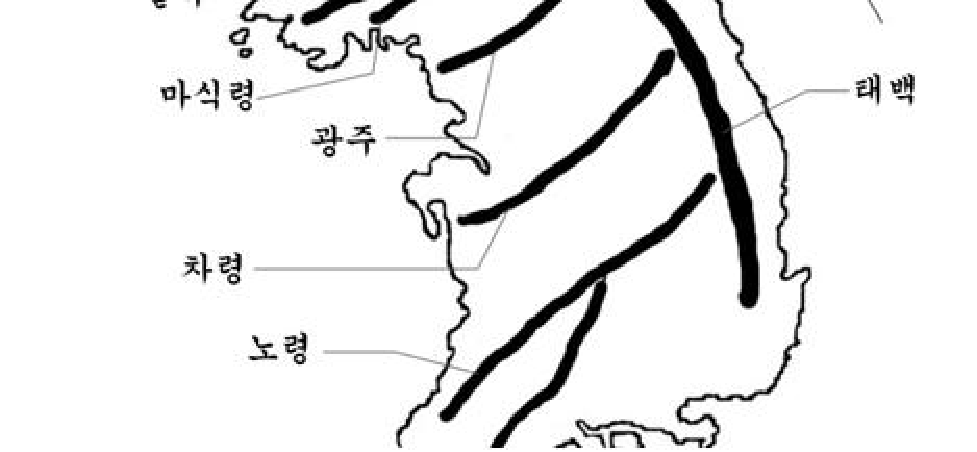
\includegraphics[width=1.0\textwidth]{./fig/fig__111.pdf}

【 차령산맥 】은 태백산맥의 오대산 부근에서 분기하여 남서로 뻗어 충청북도와 경기도의 도계를 이루고, 서해안의 대천과 군산 사이의 작은 섬들에까지 이르며, 그 길이는 약 200㎞이다.

【 노령산맥 】은 호남 지방의 대표적 산맥으로 소백산맥에서 갈라져 남서로 뻗어 서해안의 변산반도, 무안반도를 거쳐 목포까지 이르는 산맥이다.





이 두 산맥은 조산운동으로 이룩된 습곡산맥으로, 그 뒤 외인적인 침식·삭박 작용을 받아 노령기산맥을 이루고 있다. 아울러 계곡도 중국 방향의 종곡(縱谷)을 이루고 있음이 뚜렷하다. 



		\newpage  \null
	% -------------------------------------- page -------------------
		\subsection{2) 요동방향 산계}
		\null




요동방향산계는 동북동에서 서남서 방향으로 뻗는 산맥들로 【 강남산맥 】, 【 적유령산맥 】, 【 묘향산맥 】이 대표적이고 평안북도 산지의 골격을 이루고 있다.

				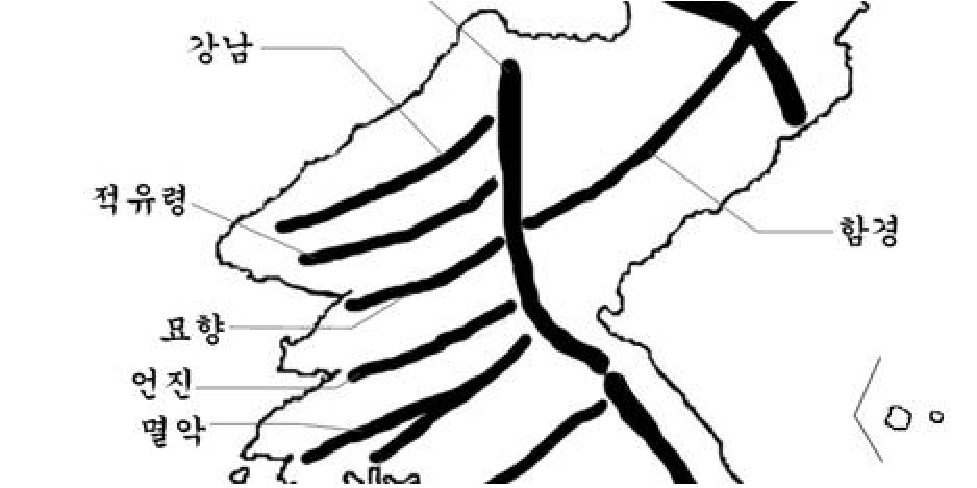
\includegraphics[width=1.0\textwidth]{./fig/fig__112.pdf}


학설에 따라서는 엄밀히 따져 요동방향은 아니나 이에 가까운 멸악산맥·언진산맥을 여기에 포함시키기도 한다. 

【 강남산맥 】은 낭림산맥의 아득령에서 갈라져, 압록강을 끼고 서남서로 달리면서 북쪽 사면이 단층절벽을 이루고 있다.

【 적유령산맥 】은 낭림산맥의 소백산에서 갈라져 강남산맥과 평행으로 달리는데, 남쪽 사면이 절벽을 이루고 청천강이 비슷한 방향으로 흐른다.

【 묘향산맥 】은 낭림산에서 갈라져 서남서로 뻗고 언진산맥은 평안남도의 주된 산맥으로 대동강을 끼고 솟는다. 

【 멸악산맥 】은 황해도의 산맥으로 재령강을 끼고 중국의 산둥성(山東省)과 마주한다.

이와 같이, 요동방향산맥은 중국방향산계와 같은 시기의 조산운동으로 생긴 습곡산맥이다. 일부 학자는 부전령산맥이나 함경산맥을 묘향산맥의 연장이라고 보는 견해도 있다.

다만, 부전령산맥과 함경산맥은 지괴운동(地塊運動)을 수반한 융기운동에 의하여 생긴 까닭으로 구조상 구별한다. 한국방향산계의 산맥들은 북북서에서 남남동 방향으로, 즉 한반도와 같은 방향의 산맥인데 일본 동경대학(東京大學)의 지질학자인 고토(小藤文次郎)에 의하여 호칭된 것이다. 고토는 우리 나라 산맥 및 지질·지형 연구에 중요한 영향을 준 학자이다.

				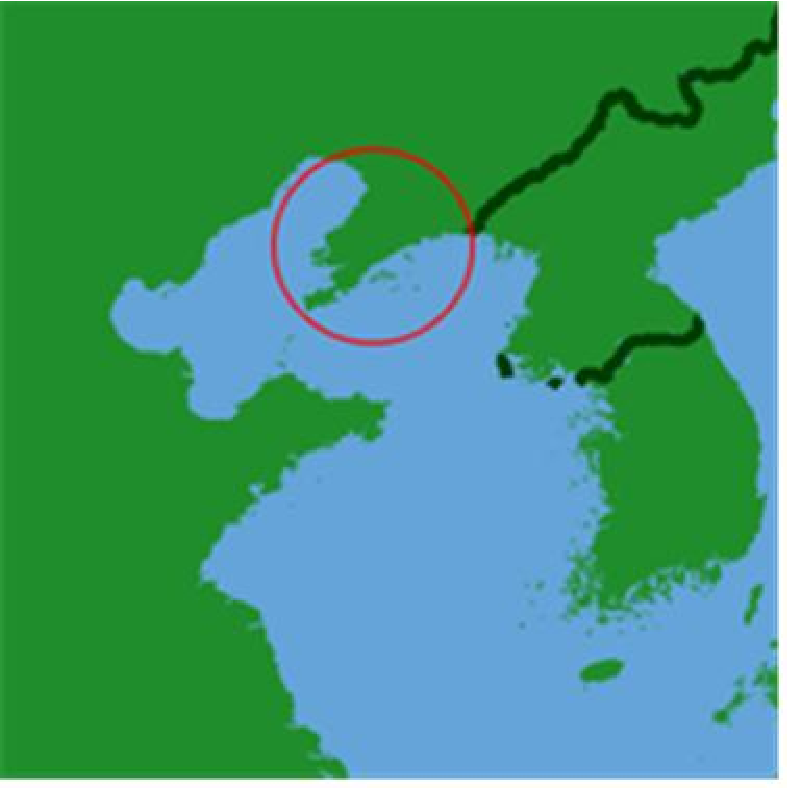
\includegraphics[width=0.6\textwidth]{./fig/fig__113.pdf}


위에 빨간색 동그라미친 부분이 랴오둥반도이며
저 부분으로 향한 산맥을 랴오둥방향이라 합니다.


		\newpage  \null
	% -------------------------------------- page -------------------
		\subsection{3) 한국방향 산계}
		\null



한국 방향의 산맥으로는 【 낭림산맥 】과 【 태백산맥 】이 있다. 

				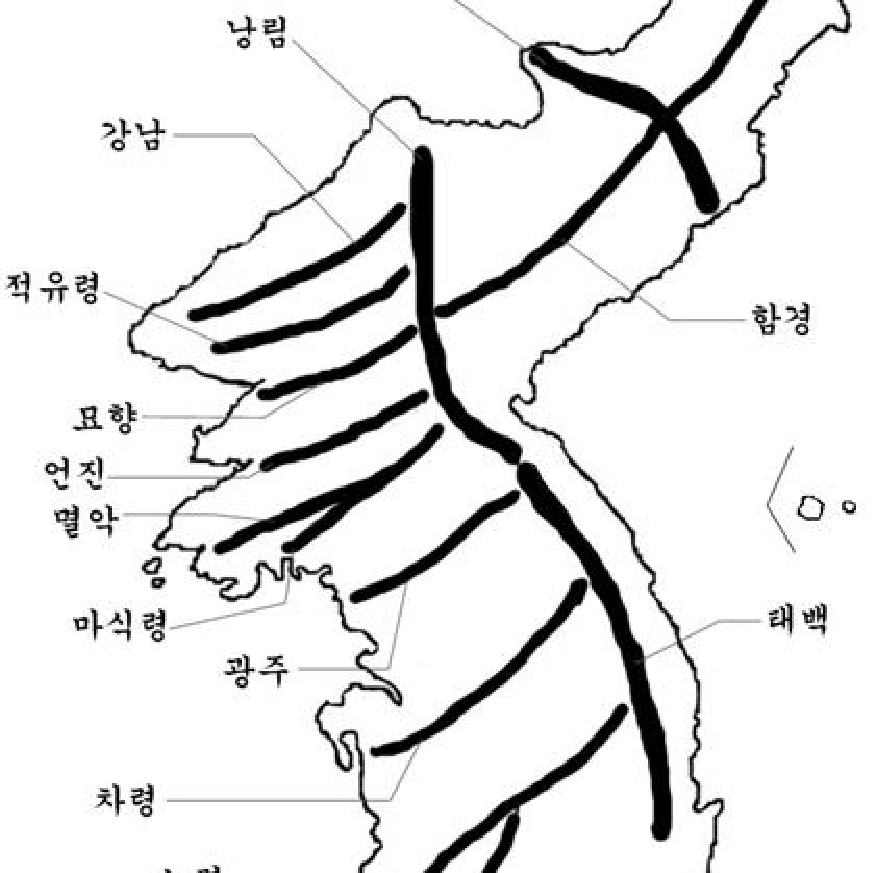
\includegraphics[width=0.6\textwidth]{./fig/fig__114.pdf}


낭림산맥은 함경도와 평안도를 경계 지은 산맥으로 중강진에서 남쪽으로 뻗어 함경산맥과 마주친다. 
태백산맥은 낭림산맥과 더불어 한반도의 척추 산맥으로 동해안을 끼고 남으로 뻗어 낙동강 하구까지 500㎞나 되는, 우리 나라에서 가장 긴 산맥이다.


낭림산맥은 단층애(斷層崖)가 서쪽을 향하고 있고, 태백산맥은 동쪽이 급사면을 이루고 있어 구조상의 차이를 보이고 있다. 마천령산맥도 대체로 한국방향산계와 같은 방향으로 뻗어 여기에 속하지만, 지질구조상 화산대산계를 이루어 태백산맥과 구별된다.


		\newpage  \null
	% -------------------------------------- page -------------------
		\subsection{4) 교차산계}
		\null




이상과 같은 세 방향의 산맥 이외에도 교차산계(交叉山系)로 보는 마식령산맥은 중국방향에 가깝지만, 작은 규모의 산맥과 교차하여 지형적으로 복잡한 형태를 이루고 있다. 소백산맥도 대체로 중국 방향이지만 동서 방향의 여러 산맥이 교차하는 까닭으로 중국방향산맥으로 보지 않고 교차산계로 따로 분류하기도 한다.

이 밖에도 함경북도를 북서로 달리다가 북북서로 뻗는 함경산맥은 2,000m의 높이를 가지는 72개의 고산군으로 함경산맥과 부전령산맥을 구분해서 보는 경우도 있다. 또한, 광주산맥은 중국 방향의 산맥으로 포함시키기도 하나, 다른 중국 방향 산맥과 지형구조상의 차이가 있어서 별도로 구분하기도 한다.

산맥 중에는 내인적(內因的)인 요소 중의 하나인 화산활동에 의해 분출된 화산맥(火山脈)이 있는데, 마천령산맥은 백두화산맥과 함께 달리며, 백두화산맥은 백두산을 비롯하여 대연지봉·간백산·북포태산 그리고 칠보산 등 여러 화산을 분출시키고 다시 울릉도·대마도(對馬島)를 지나 제주도로 이어진다.

우리 나라의 산맥은 오랜 지질시대를 거쳐 형성되었다. 

우리 나라를 포함한 아시아의 중국대륙 주변의 지사(地史)는 크게 보아 고생대는 조륙운동시기이며, 이 때 육지가 형성되었다.

중생대는 조산운동시기이고, 신생대 제3기 중엽은 지괴운동시기이며, 제3기말에서 제4기 홍적기에는 화산활동이 일어났다. 이러한 변동을 거쳐 오늘날의 산맥 지형이 형성되었다.

특히, 중생대 이후의 지각운동이 현재의 산맥 형성에 직접적인 영향을 주었다. 중생대 지각운동의 대표적인 것은 삼첩기(三疊紀) 중엽의 【 송림운동 】(松林運動)과 쥐라기 말의 【 대보운동 】(大寶運動)이다. 송림운동은 요동방향의 산맥 형성에 영향을 주었고, 충상단층(衝上斷層)이 일어나 지질구조상의 큰 변화를 일으켰다.

대보운동은 한국지사상 가장 큰 조산운동으로 심한 습곡산맥이 생기고 중국 방향의 차령산맥·노령산맥·소백산맥의 일부가 생성되었다. 요컨대, 송림운동은 북한 지방의 산맥을 생성했고, 대보운동은 남한의 주요 산맥을 생성하였다. 대보운동에 따라 화산운동이 격심해지고 화강암의 암장이 분출하여 중국 방향 산맥 형성에 큰 영향을 끼쳤다.

그 뒤 선신세에 지배사융기(地背斜隆起)의 요곡운동(墝曲運動)으로 동해안의 산맥이 생기고, 이에 따른 지괴운동으로 단층작용이 수반되어 태백산맥의 동해안쪽에 대단층선이 형성되었다. 그 뒤 신생대에는 화산활동으로 화산이 분출하여 백두화산맥이 형성되고 용암대지도 더불어 형성되었다.

이러한 내적 요인 외도 산맥은 암석에 따른 차별침식과 풍화작용, 기후에 따른 파쇄작용 등의 외적 요인에 의해 현재와 같은 지형을 보여준다. 학설에 따라서는 고전적인 조산운동이론인 대륙이동설·아이소스타시설(Isostasy說)·대륙수축설 등으로, 최근에는 지각과 맨틀 상층부의 대류이론인 판(plate)구조론으로 설명하기도 한다.

		\newpage  \null
	% -------------------------------------- page -------------------
		\subsection{참고문헌}
		\null

		\begin{itemize}[itemsep=0.0em]
		\item	『산경표(山經表)』
		\item	『조선의 산수(山水)』(최남선, 동명사, 1947)
		\item	「한국산악간지도설(韓國山嶽幹支圖說)」(이은상, 『민족문화논총』, 1973)
		\item	『신한국지리(新韓國地理)』(강석오, 새글사, 1974)
		\item	『한국의 산천』(손경석, 세종대왕기념사업회, 1975)
		\item	『한국지리총론(韓國地誌·總論)』·(건설부국립지리원, 1980)
		\item	(네이버 지식백과) 산맥 [山脈] (한국민족문화대백과, 한국학중앙연구원)
		\end{itemize}







	% ------------------------------------------ section ------------ 
	\SectionMargin
	\section{산 경 표}
	\null



1. 		산경표

산은 물을 건너지 못하고 물은 산을 넘지 못한다는 대원칙은 우리나라의 전통적 산지 인식 체계를 정리한 《산경표》의 핵심이다.

산 맥 일 반











	% ------------------------------------------ section ------------ 
	\SectionMargin
	\section{산맥}
	\null


		\newpage  \null
	% -------------------------------------- page -------------------
		\subsection{1. 산맥 [ 山脈 ]  일반}
		\null


		정의 : 산악들이 선상이나 맥상(脈狀)으로 줄지어 솟아 있는 형태의 산지 지형.
		
				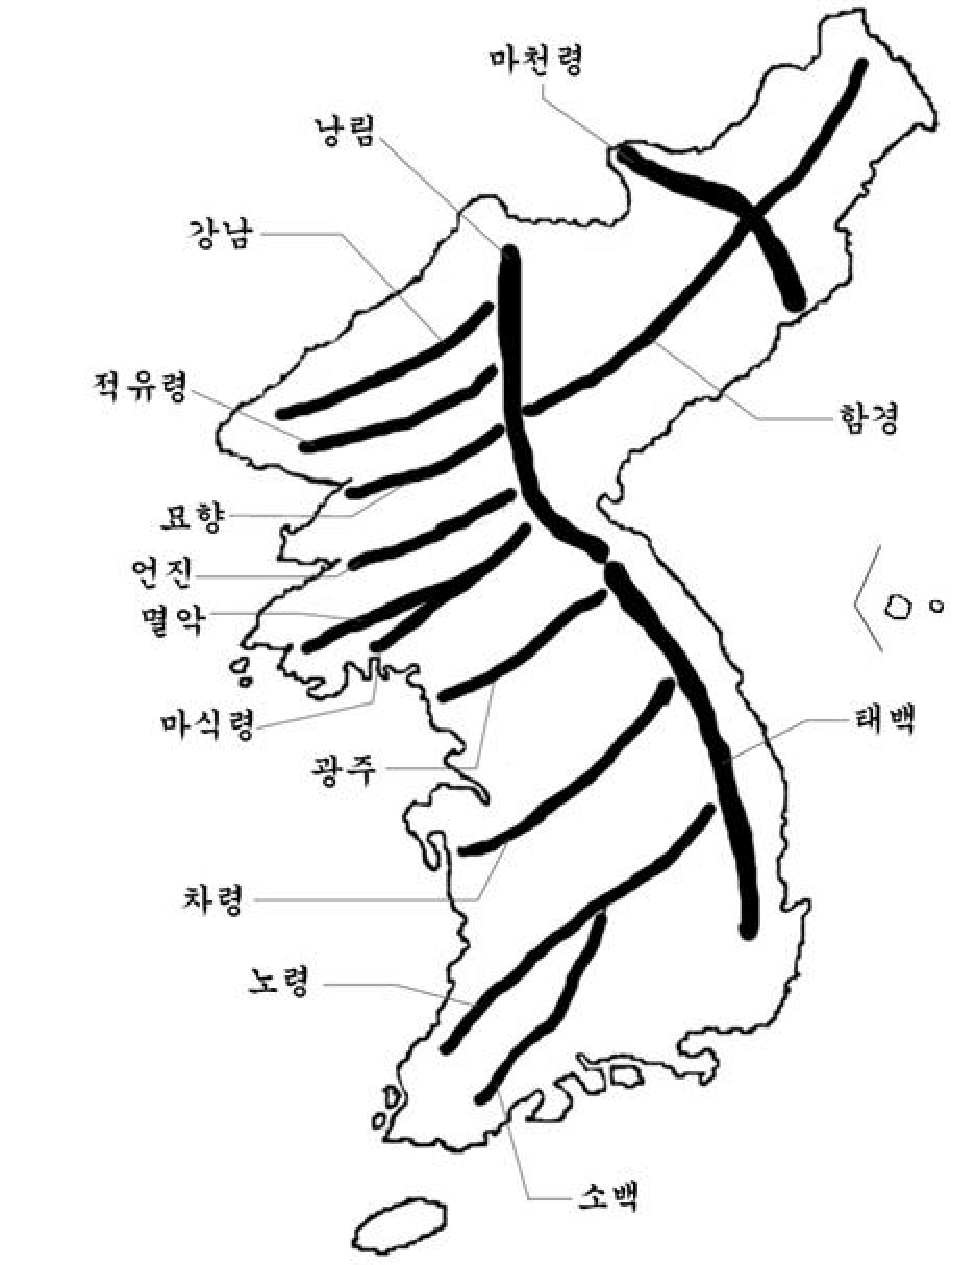
\includegraphics[width=0.8\textwidth]{./fig/fig__121.pdf}



		\newpage  \null
	% -------------------------------------- page -------------------
		\subsection{2. 산맥지도}
		\null

				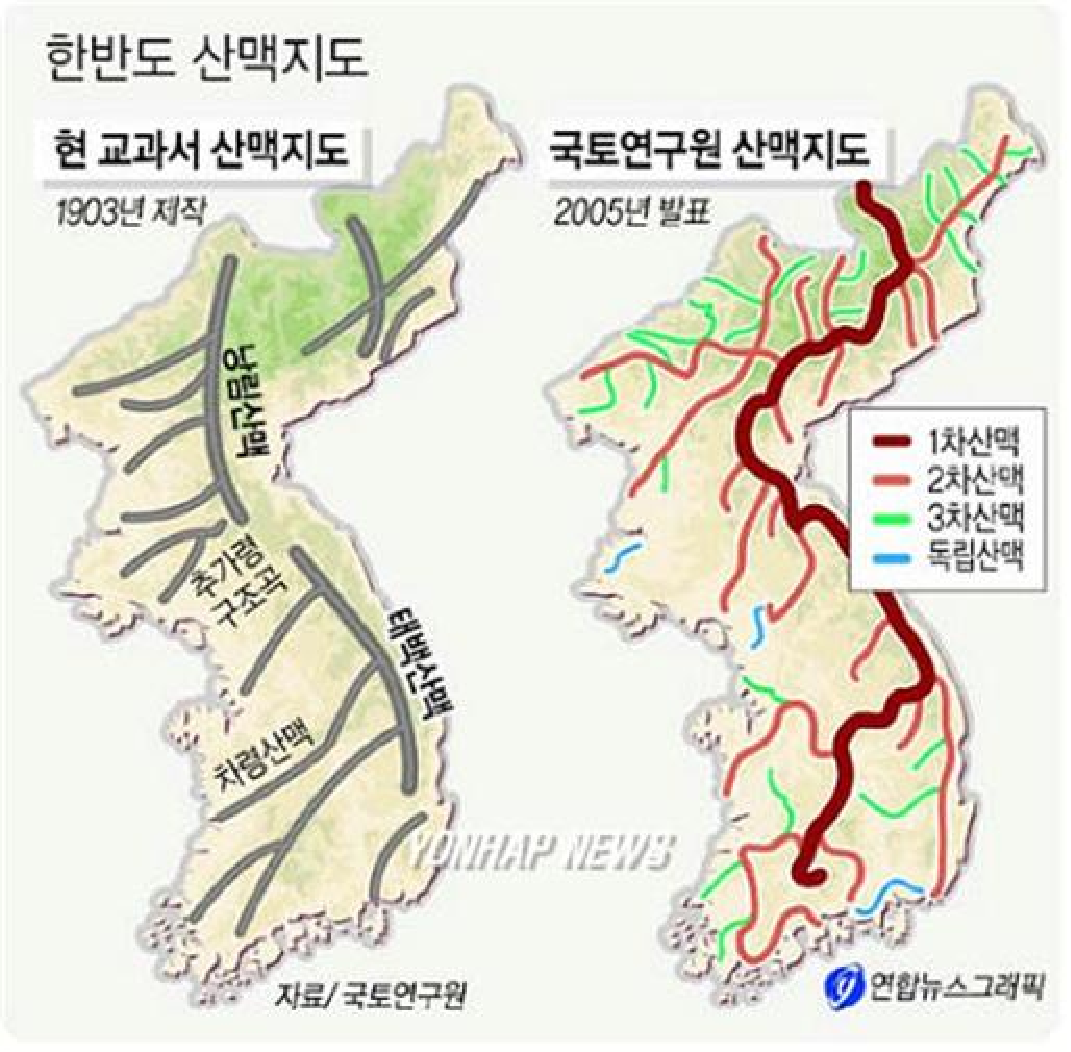
\includegraphics[width=1.0\textwidth]{./fig/fig__122.pdf}


		\newpage  \null
	% -------------------------------------- page -------------------
		\subsection{3. 내용}
		\null




보통 산지 지형은 산계(山系)·산휘(山彙)·산괴(山塊)·산맥·산령(山嶺)·산릉(山稜)·산봉(山峰)·산정(山頂) 등으로 구별되기도 하나, 산맥은 산정·산령·산봉이 계곡과 배열되어 거의 선상 또는 맥상일 때의 총칭이다. 

【 산계 】는 산맥들의 모임을 말하며 산맥에 따라서는 큰 명칭 속에 작은 산맥을 경험적으로 칭하여 포함하기도 한다.
. 

		\newpage  \null
	% -------------------------------------- page -------------------
		\subsection{4. 산맥의 구분과 명칭}
		\null




오늘날 사용되는 산맥의 구분과 명칭은 대체로 한말에 일본의 고토 등 외국인 지질·지리학자에 의해 명명되었다. 


조선 시대는 산경(山經)이라 하였는데 ≪세종실록≫ 지리지에는 구체적인 산경이 표기되지 않았다. 그 뒤 ≪동국여지승람≫이 편찬되고 ≪대동여지도≫가 김정호(金正浩)에 의해 제작되면서 한국의 산맥은 산경이라는 명칭으로 사용되었다.

영조 때의 실학자인 신경준(申景濬)이 작성한 ≪산경표 山經表≫에 의하면, 백두대간(白頭大幹)은 마천령산맥·함경산맥·서남부낭림산맥·태백산맥·소백산맥을 총칭하고, 함경산맥 북동부를 장백정간(長白正幹)이라 하는데, 간(幹)은 기본이 되는 큰 줄기를 말한다.

청천강을 경계로 북부를 청북정맥(淸北正脈), 남부를 청남정맥(淸南正脈)이라 하고, 청남정맥의 남쪽으로 해서정맥(海西正脈)·임진북예성남정맥(臨津北禮成南正脈)·한북정맥(漢北正脈)·낙동정맥(洛東正脈)·한남정맥(漢南正脈)·금북정맥(錦北正脈)·금남정맥(錦南正脈)·호남정맥(湖南正脈) 등 정맥 호칭을 붙였다.

또한, ≪산리고 山里攷≫라는 기봉방역지(箕封方域誌)에는 백두대간을 중심으로 산맥 이름에 고유 명칭을 써서 불렀다. 이은상(李殷相)은 이를 토대로 해서 한국산악간지도설(韓國山嶽幹支圖說)을 주창했는데, 조산(祖山)인 백두산을 시원(始源)으로 해서 백두대간을 한반도의 척량(脊梁)으로 치고, 이 중 북부고지와 동부고지·남부고지 등 셋으로 구분했다.

북부고지백두대간은 백두산에서 안변의 박달령(朴達嶺)에 이르는 큰 산줄기를 말하고, 동부고지백두대간은 안변의 박달령에서 봉화의 태백산까지의 큰 줄기를 말하며, 남부고지백두대간은 다시 태백산에서 김해에 이르는 큰 줄기로, 이 세 줄기를 총칭하여 백두대간이라 하였다. 즉, 오늘날의 마천령산맥·낭림산맥·태백산맥·소백산맥 일부를 총칭한 한반도 중심 골격 산맥을 설명했다.

지맥으로는 낙동강 동쪽 고지를 타고 내려간 태백산에서 부산의 동래까지의 산맥을 낙동고지태백간지(洛東高地太白幹支)로 치고, 오늘날의 태백산맥 남부를 뜻하였다. 한편, 한반도 동부의 오늘날의 함경산맥에 해당되는 줄기는 관북고지장백간지(關北高地長白幹支)로 호칭하고, 소백산맥 남부에 해당하는 산맥은 호남고지장안간지(湖南高地長安幹支)로 불렀다.

한편, 금강을 중심으로 금강 북쪽 산지를 금북고지속리간지(錦北高地俗離幹支)로 부르고, 남쪽은 금남고지마이간지(錦南高地馬耳幹支)로 불렀다. 북은 속리산을 중심으로 한 금강 북쪽, 즉 오늘날의 소백산맥 일부이고, 남은 마이산을 중심으로 한 부여까지의 줄기를 말하였다.

또한, 한강을 경계로 한강 북쪽, 즉 오늘날의 광주산맥은 한북고지분수간지(漢北高地分水幹支)라 하고, 한강 남쪽의 속리산에서 금북고지를 타고 내려오다 칠현산(七賢山)에 이르러 한강 남쪽의 통진·김포 사이의 문수산(文殊山)까지의 차령산맥 일부를 포함한 산맥을 한남고지칠현간지(漢南高地七賢幹支)로 불렀다.

임진강 북쪽의 고지 줄기는 임북고지개련간지(臨北高地開蓮幹支)로 불러 개련산을 중심으로 임진강 북쪽 산지를 말했다. 또한, 예성강 서쪽 산줄기를 예서고지개련간지(禮西高地開蓮幹支)로 불러 역시 예성강과 개련산을 연관시켜 말했다.

평안도 산지는 청천강을 경계로 그 북쪽의 여러 산지를 청북고지낭림간지(淸北高地狼林幹支)로 호칭하고 오늘날의 묘향산맥·언진산맥, 북으로 적유령산맥을 포함시켰다.

대체로, 강을 경계로 산지를 산맥 줄기나 지질구조와는 상관하지 않고 시계(視界)나 목측(目測)으로 산지 경관을 호칭한 경향이 있다. 백두산을 나라의 중심 기원 조산으로 삼은 대간 호칭은 역사적으로나 지리적으로 뜻이 있다고 생각되며, 이 대간 외 간지나 정맥·지맥으로 호칭한 것이 흥미롭다.

또한, 산맥의 호칭과 지역 구분의 특성은 일제 강점기 때의 명명에서 벗어나 새로운 시도가 요구된다. 아울러 구월산맥(九月山脈)·가야산맥(伽倻山脈)·능주산맥(綾州山脈)·수양산맥(首陽山脈)·연화산맥(蓮花山脈)·지리산맥(智異山脈)같이, 비록 규모는 작지만 지맥의 호칭이나 다른 산맥에서 확실히 분리된 지형구조의 산맥들은 정리, 확정되어야 할 것이다.




		\newpage  \null
	% -------------------------------------- page -------------------
		\subsection{차 령 산 맥[ 車嶺山脈 ] }
		\null



			태백산맥의 오대산(五臺山)에서 갈라져서 충북의 북부, 충남의 중앙을 남서 방향으로 뻗은 산맥.  

				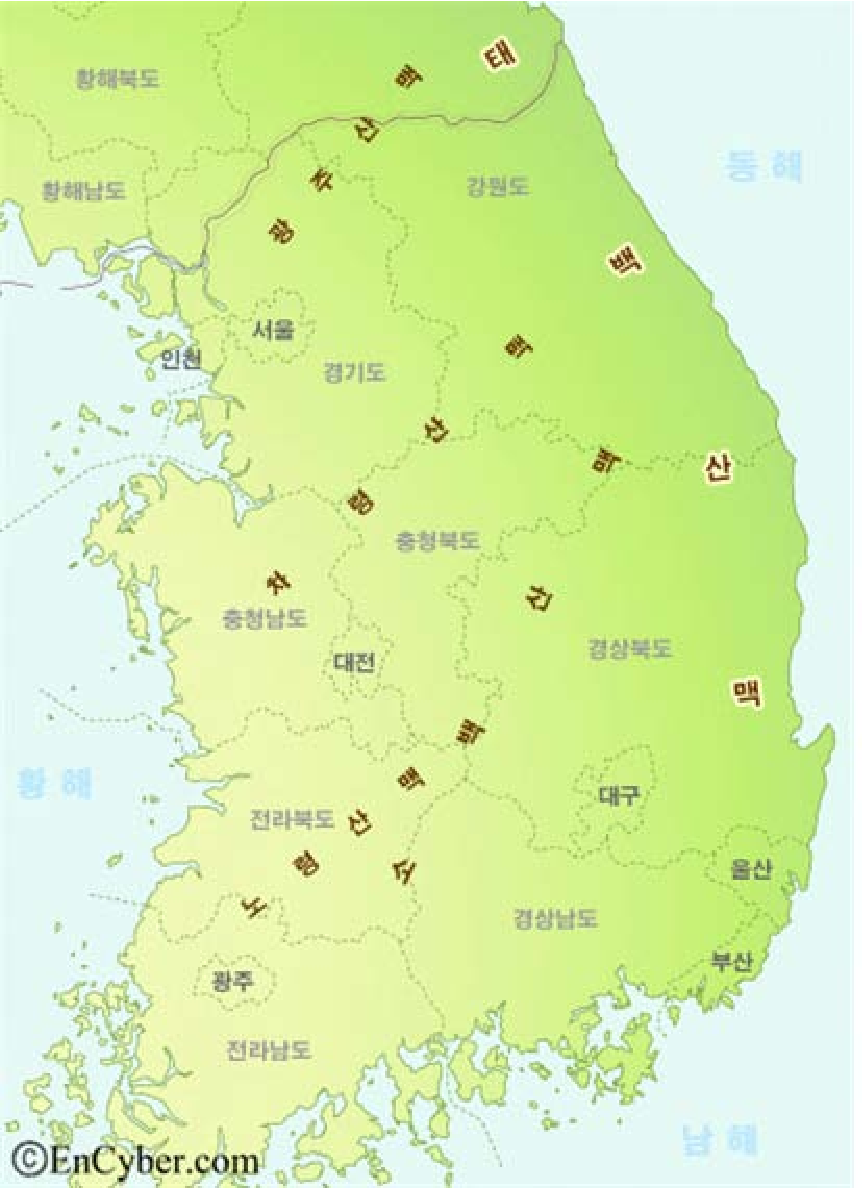
\includegraphics[width=0.6\textwidth]{./fig/fig__124.pdf}



			(1) 위치 
			태백산맥의 오대산(五臺山)에서 갈라져서 충북의 북부, 충남의 중앙 
			
			(2) 높이 
			평균고도 600 m 

길이 250 km. 평균고도 600 m. 마식령(馬息嶺) ·광주(廣州) ·소백(小白) ·노령(蘆嶺)산맥 등과 함께 한국에서 가장 오래 된 중생대 말의 습곡산맥으로 편마암과 화강암으로 구성된 구릉성 산지이다. \\

또 차령산맥은 최한월(最寒月) 평균기온 -3 ℃의 등온선과 일치하여 한국의 기후구를 남부의 온대와 북부의 냉대로 크게 구분하는 경계가 되고 있다. \\

산맥 중에는 차령 ·백운산(白雲山) ·만뢰산(萬籟山) ·칠갑산(七甲山) ·금계산(金鷄山) ·서운산(瑞雲山) 등이 솟아 있고 금 ·은 ·중석 등이 매장되어 있다. 특히 칠갑산을 중심으로 한 일대는 경치가 아름다워 1973년 충남 도립공원으로 지정되었다. 
 













% ========================================== chapter ============ 트리즈
\newpage
\chapter{습곡대}

	퇴적 지역에 강한 습곡 작용으로 형성된 습곡 지대를 말한다.  

	\SectionMargin
	\section{	습곡대 [ folded belt, 褶谷帶 ] }

		습곡은 원래 판상이었던 퇴적 구조가 지구조의 조산운동으로 휜 것으로 
		일반적으로 변형 작용으로 생성된 것을 가리킨다. 
		오목한 부분을 【 향사 】, 불룩한 부분을 【 배사 】라 한다. 향사에는 신기의 암층이 존재한다.

		\newpage
		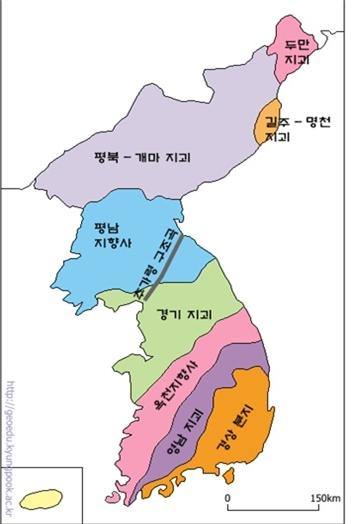
\includegraphics[width=1.0\textwidth]{./fig/belt-001.jpg}	


■ 습곡대
	\begin{enumerate}[itemsep=-0.5em]
	\item[]	한반도 지형을 보면 육괴와 육괴(지괴) 사이는 오목한 퇴적 분지( 평남 지향사, 옥천 지향사)가 대체로 좁고 길게 존재한다. 
			이곳에 퇴적 작용으로 쌓인 퇴적층에 지각 변동에 따른 횡압력이 작용하면 넓은 범위에 걸쳐 습곡으로 변형된 지형이 생긴다. 
			이러한 습곡 지역을 【 습곡대 】라 한다. 
	\item[]	
	\item[]	우리나라의 선캄브리아대 습곡대는 대체로 오랜 시간 동안 압력에 따른 변형으로 변성암화된 지층이 거의 다수를 차지한다.
	\item[]	
	\item[]	한반도의 대표적인 습곡대로는 【 함북(두만강) 분지 】, 【 단천 습곡대 】, 【 평남 분지 】, 【 옥천 습곡대 】, 
			【 경상 분지 】, 【 포항(연일) 분지 】등이 존재한다. 
	\item[]	
	\item[]	단천 습곡대는 선캄브리아대에 함북 분지에 퇴적되었고, 평남 분지와 옥천 습곡대는 고생대에 퇴적되었으며, 
			경상 분지는 중생대에, 포항(연일) 분지는 신생대 제3기에 퇴적된 것으로 밝혀졌다.
	\item[]	
	\item[]	습곡대 존재의 예로 【 옥천 습곡대 】는 경기 육괴와 영남 육괴 사이에 대상(帶狀)으로 분포하고, 
			【 평남 습곡대 】는 평북 육괴와 경기 육괴 사이에 존재한다.
	\item[]	[네이버 지식백과] 습곡대 [folded belt, 褶谷帶] (두산백과)
	\end{enumerate}




% ========================================== chapter ============ 
\newpage
\chapter{지 향 사[ geosyncline, 地向斜 ]}


	\SectionMargin
	\section{	지향사 [ geosyncline, 地向斜 ] 일반 }



	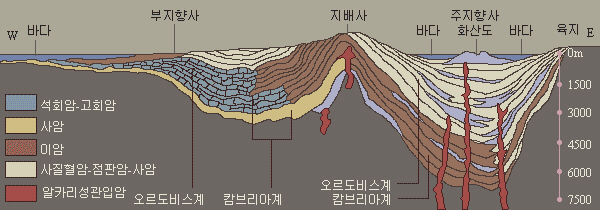
\includegraphics[width=1.0\textwidth]{./fig/geosyncline-001.jpg}	


	\subsection{지향사}

		막대한 양의 퇴적물이 쌓이는 지표면의 대규모 침강지대를 말한다. 
		\\[-1.0em]

		일반적으로 지향사는 화산암류가 많고 심해저퇴적물이 쌓여서 된 완지향사와, 
		화산암류가 없고 비교적 천해층퇴적물이 쌓여서 된 차지향사로 이루어져 있다.  
		\\[-1.0em]

		완지향사
		차지향사

		지향사 
		지각의 일부가 침강하면서 퇴적암과 화산암이 수 km의 두께로 쌓이는 수 km 이상의 길쭉한 퇴적분지. 

		지향사 
		지구의 표면에서 대규모로 침강·퇴적하고 있는 지역. 



	\SectionMargin
	\section{	지향사에 대한 이론}

	\subsection{지향사}

		1859년 J.홀이 처음으로 지향사에 대한 이론을 발표하였다. 
		\\[-1.0em]

		홀은 아메리카대륙 동안(東岸)에서 서부의 미시시피강에 이르는 내륙평원의 단면을 그리던 중, 
		각 지층이 애팔래치아산맥 부근에서 서쪽 평원지구에 비해 몇 배에서 십여 배나 두꺼운 것을 발견하고 
		이러한 두꺼운 지층이 습곡작용(褶曲作用)을 받아 융기하여 산맥을 만든다고 주장하였다. 
		\\[-1.0em]

		그후 1873년 J.W.데이너가 습곡산맥을 만드는 두꺼운 지층이 형성되는 지대를 지향사라고 명명하였다. 
		데이너는 지향사가 대륙과 해양의 경계를 따라 분포하며, 
		거기서 생기는 습곡대(褶曲帶)가 화강암의 관입(貫入)으로 해양을 잠식하며 대륙을 바깥쪽으로 성장시키는 것으로 생각하였다.
		\\[-1.0em]

		현재, 지향사는 대지지역(臺地地域)에 대치되는 지각의 중요한 구조단원의 하나로서, 다음과 같은 특징을 가지고 있다. 
		퇴적층이 띠 모양으로 배열되어 있고, 격렬한 습곡작용과 활발한 화성활동(火成活動)이 일어난다. 
		이러한 지각활동으로 광역변성작용이 나타나고, 특수한 광화작용(鑛化作用)에 의해서 많은 광상(鑛床)이 생성된다.
		\\[-1.0em]

		지향사의 초기단계에는 전역에 걸쳐 침강이 탁월하여 1만∼1만 5000m에 이르는 두꺼운 퇴적층이 생긴다. 
		이에 따라 염기성마그마의 분출과 관입이 일어난다. 
		다음의 발전단계에서는 화강암류의 관입이 강화되고, 곳에 따라 습곡과 융기가 일어나며, 융기부가 새로 침강한다. 
		이어서 모든 지역에 퇴적이 중단된다. 
		말기단계에서는 습곡작용이 한층 격화하고, 대규모의 화강암 관입과 지향사 전역에 융기가 일어나서 습곡산맥이 형성된다. 



	\subsection{지향사 [ 地向斜, geosyncline ] }


		장기간에 걸친 침강이 계속되어 두꺼운 지층이 퇴적된 지역을 말한다. 

		홀(T. Hall, 1859)이 애팔래치아 산지의 연구에서 제창하고, 다나(J. D. Dana)가 명명하였다. 
		홀과 다나는 내륙 주변의 얕은 바다를 생각하였으나, 하우그(E. Haug, 1960)는 대륙과 대륙 사이의 깊은 바다를 생각하였다. 
		그 후 많은 학자들의 연구에 의해 여러 가지 형태의 퇴적지역에 사용하게 되었고 그 내용도 매우 다양하게 되었다. 
		보통 수백 ㎞ 이상의 넓이를 갖고 수천 m의 지층이 퇴적된 경우를 말하지만 훨씬 소규모의 퇴적분지에 적용하기도 한다. 
		그 성인의 메커니즘에도 지각변동 학설의 진전에 따라 다양한 해석이 가능하게 되었다. 

		최근 해양조사의 현저한 진보와 판구조론의 진전에 따라 지향사의 개념에 뚜렷한 변화가 일어나고 있다. 
		오늘날 세계적인 대산맥들 가운데 두꺼운 퇴적층이 존재하는 곳은 그곳이 과거 지질시대에 지향사였음을 시사하는 것이다. 
		한편 서해, 동지나 해, 남지나 해, 동해, 오호츠크 해를 연결하는 긴 지대 및 지중해, 멕시코 만 등은 
		현재 계속 퇴적물이 쌓이고 있는 소위 ‘살아 있는 지향사’라고 할 수 있다. 

		지향사는 규모, 지역성, 퇴적시기, 화산활동, 조산운동 등의 관계를 고려하여 여러 가지 형태로 분류된다. 
		슈체르트(C. Schuchert, 1923), 스틸(H. Still, 1936)을 거쳐 케이(M. Key, 1947)가 정리한 지향사의 분류는 다음과 같다.

		\begin{enumerate}
		\item[①]	정(正)지향사 : 대륙 사이에 발달한 것으로 알프스와 같은 조산대를 만든 지향사 
				\begin{enumerate}
				\item[㉠] 완(完)지향사→화산활동을 동반, 
				\item[㉡] 차(次)지향사→화산활동을 동반하지 않음
				\end{enumerate}
		\item[②] 준(準)지향사 : 내륙에 발달한 것으로 조산대를 형성하지 않은 지향사 
				\begin{enumerate}
				\item[㉠] 외(外)지향사→정지향사가 설상(舌狀)으로 연장된 것, 
				\item[㉡] 내(內)지향사→내륙에 고립된 지향사, 
				\item[㉢] 종(從)지향사→내륙에서 융기하는 곳에 접하여 보정(補正)역할로 침강한 지대.
				\end{enumerate}
		\end{enumerate}

		(자연지리학사전, 2006.5.25, 한울아카데미)


	\SectionMargin
	\section{옥천 지향사}








	\SectionMargin
	\section{평남 지향사}




% ========================================== chapter ============ 
\newpage
\chapter{조 산 운 동}




	\SectionMargin
	\section{	조산운동 일반}

		대규모의 습곡산맥을 형성하는 지각변동.



	\SectionMargin
	\section{	조산운동의 과정}

		조산운동의 과정은 【 지향사(地向斜)단계 】, 【 조산 단계 】, 【 침식 단계 】의 세 단계로 나뉜다. 

	\SubSectionMargin
	\subsection{(1) 지향사 단계}

		지향사 \footnote{막대한 양의 퇴적물이 쌓이는 지표면의 대규모 침강지대를 말한다. 
		일반적으로 지향사는 화산암류가 많고 심해저퇴적물이 쌓여서 된 완지향사와, 
		화산암류가 없고 비교적 천해층퇴적물이 쌓여서 된 차지향사로 이루어져 있다.
		[네이버 지식백과] 지향사 [geosyncline, 地向斜] (두산백과)}단계는 
		지향사에 【 퇴적층 】이 형성되는 단계이다. 
		\\[-1.0em]

		종전에는 얕은 바다에 퇴적물이 쌓이고 그 무게에 의하여 퇴적층이 침강하면 
		여기에 다시 퇴적물이 쌓여서 두꺼운 퇴적층의 지향사가 만들어진다고 보았다. 
		\\[-1.0em]

		그러나 현재의 지향사는 【 완지향사 】(完地向斜)와 【 차지향사 】(次地向斜)가 쌍을 이루며, 
		깊은 완지향사는 심해성퇴적물과 화산분출물이 쌓여서, 
		얕은 차지향사는 천해성퇴적물이 쌓여서 만들어지는데, 
		판구조론에 의하여 서서히 침강하여 그 두께가 1만 m가 넘는 퇴적층이 되는 것으로 알려져 있다. 
		\\[-1.0em]

		이와 같은 지향사는 현재 일본해구~일본~동해~아시아대륙을 연결하는 지대와, 
		자바해구~자바~남중국해~아시아대륙을 연결하는 지대가 대표적이다. 
		일반적으로 환태평양(環太平洋) 연안부가 이와 같은 지향사의 쌍을 이루는 곳이라고 본다. 




	\SubSectionMargin
	\subsection{(2) 조산 단계}
		조산단계는 지향사를 이루는 두꺼운 퇴적층이 판과 판이 【 충돌 】하거나 한 판이 다른 판 밑으로 【 침강 】할 때 
		작용하는 거대한 【 횡압력 】을 받아서 【 습곡 】(褶曲)\footnote{( 쐐기 습 굽을 곡휘어진 정도나 휘어진 양에 상관없이 암석이 휘어진 상태의 지질구조.
		습곡 작용은 양쪽 옆에서 압축하는 경우에 생겨난다.
		습곡은 일반적으로 배사와 향사라는 두 가지의 구조를 가진다. 
		배사구조(anticline)는 암석이 힘을 받아 위로 볼록하게 솟아올라 휘어진 경우이고 
		향사구조(syncline)는 반대로 접시처럼 아래로 움푹 들어가게 휘어진 경우를 말한다
		[네이버 지식백과] 습곡 [fold, 褶曲] (두산백과)}을 만들고 거대한 【 습곡산맥 】으로 되는 단계이다. 
		\\[-1.0em]

		알프스 ·히말라야산맥은 아프리카판과 인도판이 북으로 움직이며 유라시아판과 충돌하여 이루어진 대습곡산맥이고, 
		환태평양조산대는 태평양판이 아프리카판 ·유라시아판 ·인도판 밑으로 침강하여 형성된 것이다. 
		이들 습곡산맥은 무수한 단층을 가지고 있고, 
		그 축(軸) 부분은 화강암의 관입(貫人)으로 광역변성작용(廣域變成作用)을 받아 편마암이나 결정편암으로 변한 것이 대부분이다. 
		\\[-1.0em]

		좁은 뜻에서는 이 단계만을 조산운동이라고도 한다. 

	\SubSectionMargin
	\subsection{(3) 침식단계}
		침식단계는 습곡운동이 그친 후 융기된 습곡산맥이 풍화침식으로 깎이어 평탄해지는 단계이다. 
		선캄브리아기에 생성된 조산대는 평탄하게 깎이어 안정된 순상지(楯狀地)를 이루고 있고, 고생대의 습곡산맥도 몹시 깎이어 낮아져 있다. 




	\SectionMargin
	\section{	조산운동}


		고생대 이후 유럽에서 조산운동이 일어난 것은 
		고생대 중기와 말기, 중생대 말기~신생대 초기에 걸친 크게 3차례였다. 
		이들은 각기 【 칼레도니아 조산운동 】 ·【 헤르시니안 조산운동 】 또는 【 바리스칸 조산운동 】 ·【 알프스 조산운동 】이라고 부른다. 


		\begin{enumerate}[leftmargin=3cm]
		\item[1.]		칼레도니아 조산운동
		\item[2.]		헤르시니안 조산운동
		\item[3.]		바리스칸 조산운동
		\item[4.]		알프스 조산운동
		\end{enumerate}


		\subsection{북아메리카의 조산운동}			
		또한 북아메리카에서도 약간의 시기의 차는 있지만, 고생대에는 타코닉조산운동과 애팔래치아조산운동이, 
		중생대 중기에는 네바다조산운동이, 그리고 중생대 말기부터 신생대 초기에 걸쳐서 일어난 라라미드조산운동이 알려져 있다. 

		\subsection{한국의 조산운동}
		한국에서는 칼레도니아조산운동에 해당하는 것이 대결층(大缺層)으로 밝혀졌으며, 
		고생대 말기의 것은 밝혀지지 않았고, 
		아메리카의 네바다조산운동에 해당하는 것이 【 송림변동 】(松林變動)과 【 대보조산운동 】(大寶造山運動)으로, 
		라라미드조산운동에 대응하는 것이 【 불국사변동 】(佛國寺變動)으로 알려져 있다. 
		또한 대보조산운동과 불국사변동은 유럽의 알프스조산운동에도 해당하며, 중국의 옌산운동[燕山運動]과도 시기를 같이 하고 있다. 
		[네이버 지식백과] 조산운동 [orogeny, 造山運動] (두산백과)





	\SectionMargin
	\section{	송림변동 (트라이아스기)}





	\SectionMargin
	\section{	대보조산운동}

		\subsection{대보조산운동}

		중생대 쥐라기부터 백악기 초까지 우리나라 땅 전역에서 일어난 대규모 지각 변동
		평양 근처의 대보탄전의 이름을 딴 것이다.


		\subsection{대보조산운동의 어원}

		대보조산운동의 대보는 도대체 무엇인가?
		우리나라 지질, 암석, 지각 운동 등은 익숙하지 않은 명칭을 갖고 있다. 
		이름이 너무 낯설어 기억하기에도 쉽지 않다.  
		그래서 지각 운동의 이름을 좀 정리해보고자 한다. 우선 대보조산운동이 눈에 들어온다. 

		大寶造山運動 에서 대보 大寶 는 큰 보물??? 이라는 뜻인가?
		대보를 지명으로 보고 일부 지식인들은 경상북도 포항시 남구 호미곶면의 옛 이름 대보면에서 이름을 따왔다고 하나 그것을 정확한 게 아니다. 
		대보는 평양 근처의 대보탄전에서 온 명칭이다.

		\SubSectionMargin
		\textbf{대보조산운동의 어원}
		\\[-1.0em]

		대보조산운동이란 일본인 지질학자인 分野圓藏(1927)이 북한의 평양부근의 대보탄전을 조사한 후 
		일본 지리학회지인 지질학잡지에 '조선대보탄전 부근의 지질과 구조'라는 논문에서 처음으로 기재되었다고 한다. 
		\\[-1.0em]

		그는 대보탄전부근의 지질을 조사하여 대동계층과 대보층 사이에 큰 트러스트가 있으며 
		이 트러스트를 일으킨 지각운동을 '대보충동'이라고 하였고 이 시기를 대동계층이 퇴적된 후~ 대보층이 퇴적되기 전으로 보았다. 
		\\[-1.0em]

		대보조산운동은 대동계 퇴적 후 즉 쥬라기 말에, 송림변동은 그 이전인 평안계 지층의 퇴적 후 즉, 트라이아스기 말에 일어난 것으로 인정되고 있다. 

		
		\begin{enumerate}[itemsep=-1.0em]
		\item[] 원문 출처: 大寶造山運動이란 무엇이며, 그 問題點은 무엇인가? = Daebo Orogeny and its Problems 
		\item[] 학술지명 : 지질학회지(Journal of the Geological Society of Korea) 
		\item[] 권호사항 : Vol.24 No.2 [1988] 
		\item[] 발행처 : 대한지질학회 
		\item[] 발행처 URL : http://www.gskorea.or.kr 
		\item[] 자료유형 : 학술저널 
		\item[] 수록면 : 175-177(3쪽)
		\end{enumerate}






	\SectionMargin
	\section{불국사운동}




	\subsection{불국사운동}

		불국사 조산운동 혹은 불국사 변동은 기원전 9,700만 년에서 기원전 5,700만 년 사이 
		즉, 【 중생대 백악기 】부터 【 신생대 제3기 】까지 한반도에서 일어난 조산 운동이다.
		\\[-1.0em]

		중생대에 접어들면서 한반도는 대륙의 가장자리 위치해 있었기 때문에 
		침강하는 해양판으로 인해 많은 지질적인 변화를 겪게 되었다. 
		불국사 조산운동은 그로 인해 발생한 조산 운동이다. 
		이 조산운동으로 생성된 화강암을 【 불국사 화강암 】이라고 한다. 
		경주의 불국사 토함산의 화강암의 연대를 측정하여 얻은 결과, 
		다른 지역의 화강암과의 연대가 달라서 이를 불국사 화강암이라 하였는데, 화강암의 이름을 따서 불국사 조산운동이라는 이름이 붙여졌다

		불국사 운동에 의하여 한국 방향의 구조선이 형성되었으며 경상 분지가 육화되었다. 

		\paragraph{불국사 화강암}
		한편, 경상 분지를 중심으로 화산 활동과 화강암의 관입이 광범위하게 발생하였는데, 이 화강암을 불국사 화강암이라고 한다.
		[네이버 지식백과] 불국사 운동 [佛國寺運動] (Basic 고교생을 위한 지리 용어사전, 2002.2.5, (주)신원문화사)



	\subsection{설악산 울산바위}
	설악산의 울산바위는 신생대가 시작하기 약 500만 년 전에 있었던 중생대말 백악기 때 있었던 【 불국사운동 】으로 형성된 화강암이다.







	\SectionMargin
	\section{	경동성 요곡운동}




	\subsection{경동성 요곡운동}

\paragraph{경동성 지형}
산지를 이루는 지형이 한쪽은 높고 급한 면을 이루고, 다른 한쪽은 낮고 경사가 완만한 면을 이루는 지형을 【 경동성 지형 】이라 한다. 


\paragraph{경동성 요곡운동}
경동성 요곡운동이란 이러한 지형을 형성하는 요곡운동을 말하며 이렇게 형성된 산지나 지형은 결과적으로 좌·우 비대칭을 이룬다.



	\subsection{경동성 요곡운동}


경동성 요곡운동에 의해 형성된 대표적인 지형은 한반도를 들 수 있다. 

한반도의 지형은 신생대 제3기와 제4기에 걸쳐 동해의 지각이 확대되면서 작용한 횡압력으로 인해 동해안을 축으로 지반의 융기가 전개되었다. 그 결과 산지가 동쪽으로 기우는 비대칭적 지형이 형성되었는데, 이와 같이 비대칭적으로 발생하는 요곡운동을 경동성 요곡운동이라고 한다.
\\[-1.0em]

한반도의 산지가 북동쪽의 태백산맥을 근간으로 서쪽으로는 비교적 평탄한 데 반해 동쪽으로 경사가 심한 것은 바로 이 때문이다. 또 오대산·태백산과 대관령 등 한반도의 산악지대 정상부에는 곳곳에 【 고위평탄면 】이 있는데, 이 역시 한반도가 경동성 요곡운동에 의해 융기된 지형임을 말해주는 좋은 증거이다.
\\[-1.0em]

한반도의 지형은 원래 중생대 대보조산운동이 일어난 이후 오랜 세월 동안 침식작용이 일어나면서 평탄화 되었다. 그러나 경동성 요곡운동에 의해 지반이 융기하면서 평탄면은 하곡을 중심으로 활발한 침식이 이루어졌으나, 완전히 없어지지 않고 융기한 산지에 남아 있게 된 것이다.
[네이버 지식백과] 경동성 요곡운동 [傾動性撓曲運動] (두산백과)


	\subsection{경동지형}


신생대 제3기 2,300만~1,500만 년 전, 동해의 해저 지각이 확장하면서 수평으로 가해진 횡압력으로 우리나라의 지반이 높이 융기했다. 이때 융기축이 동쪽으로 많이 치우쳐 동쪽은 높이 솟아올라 급경사를 이루었고, 서쪽은 완경사를 이루어 동고서저의 경동지형이 만들어졌다.
\\[-1.0em]

태백산맥은 이때 만들어 생겨났는데, 그 허리에 자리 잡은 금강산 또한 지반의 융기로 솟아올랐다. 이 과장에서 지하 깊숙이 있던 화강암이 지표 가까이로 끌어올려 졌고, 그 결과 지표 물질들이 빠르게 깎여나갔다. 이와 같은 지반 융기를 증명해주는 지형은 옥녀봉~비로봉~일출봉~연일봉으로 이어지는 금강산의 주능선에서 찾아볼 수 있다. 이는 고생대 이후로 오랜 침식을 받아 저평화된 지형의 일부가 별다른 습곡 작용을 받지 않고 그대로 솟아올라 정상부의 완만한 구릉성 고원지대를 형성한 것이다. 
\\[-1.0em]

주 능선을 경계로 급경사를 이루는 동쪽은 상대적으로 험하고 굴곡이 많은 산세를 형성했으며, 완경사를 이루는 서쪽은 완만한 구릉성 고원의 산세를 형성하였다. 
\\[-1.0em]

그래서 서쪽의 내금강은 그윽하고 부드러운 산세가 펼쳐져 여성미가 느껴지고, 그 위로는 만폭동, 백천동, 수렴동, 장안동 등의 계속이 유유히 굽이쳐 흐른다.
\\[-1.0em]

반면 동쪽의 외금강은 경사가 매우 급하고 구룡폭포와 만물상에서 볼 수 있듯 관음연봉을 비롯해 월출봉에서 동쪽으로 뻗어 내린 채하봉과 집선봉의 암릉은 나무 한 그루 없는 낭떠러지의 모습이라 산악미의 진수를 느끼게 한다.
\\[-1.0em]
 
내금강과 외금강은 지형뿐만 아니라 기후에서도 확연히 차이가 난다. 외금강에 속하는 고성읍의 연 평균 기온은 11.0℃, 8월 평균기온은 23.6℃, 1월 평균기온은 -2.1℃이다. 그러나 내금강에 속하는 금강읍은 각각 7.2℃, 21℃, -8.5℃로 특히 겨울철 기온이 크게 차이가 난다. 그 이유는 태백산맥 줄기가 차가운 북서 계절풍을 막아주고 동해의 난류가 영향을 미쳐 외금강의 고성읍은 온화한 해양성 기후를 보이지만, 내금강의 금강읍은 대륙성기후의 영향을 받아 춥기 때문이다.
\\[-1.0em]

연 평균 강수량은 고성군이 1,580mm 금강군이 1,201 mm 로 동해 쪽에 있는 외금강은 눈과 비가 더 많이 내린다. 이는 동해를 지나 불어오는 북동기류가 수증기를 머금고 이동하다가 백두대간의 산줄기에 부딪혀 단열팽창한 결과 수증기가 응결되어 비와 눈으로 내리기 때문이다.


	\SubSectionMargin
	\subsection{동고서저 지형이 만들어지는 과정}


한반도는 중생대에 여러 차례의 화산 활동으로 대규모 지각 변동을 겪은 후, 오랜 세월 침식과 풍화로 평탄화되어 준평원 지형을 유지하다가 신생대 제3기 중기 이후 다시 한 번 큰 격변을 겪는다. 당시 한반도의 산지 지형은 지구를 덮고 있는 여러 개의 지각판 가운데 유라시아 대륙 지각판과 태평양 지각판이 수렴, 충돌하는 지대에서 직간접적으로 전달되는 횡압력에 큰 영향을 받았다. 지금부터 2,300만~1,500만 년 전 태평양 지각판과 유라시아 대륙 지각판의 충돌로 대륙에 붙어 있던 일본 열도가 남쪽으로 떨어져 나가면서 그 사이에 저지대 분지인 새로운 해양 지각이 형성되었다. 그리고 이 분지에 해수가 밀려들어오면서 동해가 생겨났다. 이후 동해 지각 중심부의 연약대를 따라 해저가 점차 확장되었는데, 이때 수평으로 가해진 횡압력이 한반도가 있는 대륙의 서쪽 연변부를 들어올렸다. 이 과정에서 융기축이 동쪽으로 치우쳐 동해안 쪽은 급경사를 이루었고, 황해안 쪽은 완경사를 이루는 동고서저의 경동(傾動)지형이 만들어졌다. 낭림산맥, 함경산맥, 태백산맥 등 동쪽의 높은 산맥은 모드 이렇게 생겨난 것들이다.











































% ========================================== chapter ============ 트리즈
\newpage
\chapter{운동}












% ========================================== chapter ============ 트리즈
\newpage
\chapter{참고자료}


		\SectionMargin
		환경지질연구정보센타
		\url{http://ieg.or.kr/edu/edu_data_lecture.html}









































\end{document}